\documentclass[10pt]{article}
\usepackage[utf8]{inputenc}
\usepackage[swedish]{babel}

\def\ordf{Erik Månsson}
\def\sekr{Johan Karlberg}
\def\sreordf{Pontus Landgren}
\def\fvc{Sophia Grimmei\ss\ Grahm}

\def\doctype{Handlingar} %ex. Kallelse, Handlingar, Protkoll
\def\mname{Vårterminsmötet} %ex. styrelsemöte, vårterminsmöte
\def\mnum{VT/17} %ex S02/16, E01/15, VT/13
\def\date{2017-05-02} %YYYY-MM-DD
\def\docauthor{\sekr}

\def\mtime{17:15}
\def\place{E:B}

\usepackage{../../_sektion-handlingar/e-handlingar-sek}
\usepackage{../../e-mote}
\usepackage{../../../../e-sek}

\begin{document}

\firstpage{{\doctype} till {\mname} {\mnum}}{{\date} {\mtime} i {\place}}

\tableofcontents
\newpage

\subfile{../../_sektion-handlingar/_other/guide}
\newpage

\section{Dagordning}
\subsection{Tid och plats}
\tidplats

\subsection{Föredragningslista}
\begin{paralist}
    \pli{TaFMÖ}{}
    \pli{Val av mötesordförande}{}
    \pli{Val av mötessekreterare}{}
    \pli{Godkännande av tid och sätt}{}
    \pli{Val av två justeringspersoner}{}
    \pli{Adjungeringar}{}
    \pli{Godkännande av dagordningen}{}
    \pli{Föregående sektionsmötesprotokoll}{}
    \pli{Meddelanden}{}
    \pli{Beslutsuppföljning}{}
    \pli{Utskottsrapporter}{}
    \pli{Uppföljning av verksamhetsplan}{}
    \pli{Ekonomisk rapport}{}

    \pli{Val}{}
        \begin{paralist}
            \pli{Val av funktionärer}{}
            \pli{Val av hedersmedlemmar}{}
        \end{paralist}
    \pli{Verksamhetsberättelser för 2016}{}
    \pli{Bokslut för 2016}{}
    \pli{Revisionsberättelse för 2016}{}
    \pli{Styrelsens förslag till resultatdisposition}{}
    \pli{Uttag ur sektionens fonder sedan förra terminsmötet}{}
    \pli{Frågan om ansvarsfrihet för 2016}{}
        \begin{paralist}
            \pli{Funktionärer}{}
            \pli{Utskott}{}
            \pli{Styrelse}{}
            \pli{Revisorer}{}
            \pli{Valberedning}{}
        \end{paralist}

    \pli{Behandling av motioner}{}
        \begin{paralist}
            \pli{}{}
        \end{paralist}
    \pli{Behandling av propositioner}{}
        \begin{paralist}
            \pli{}{}
        \end{paralist}
    \pli{Övrigt}{}
    \pli{TaFMA}{}
\end{paralist}

\begin{signatures}{2}
    \emph{I Sektionens tjänst}
    \signature{\ordf}{Ordförande}
    \signature{\sekr}{Kontaktor}
\end{signatures}

\begin{comment} %TODO
\subfile{../_other/ekonomisk_rapport}
\newpage
\addcontentsline{toc}{subsection}{Balansrapport}
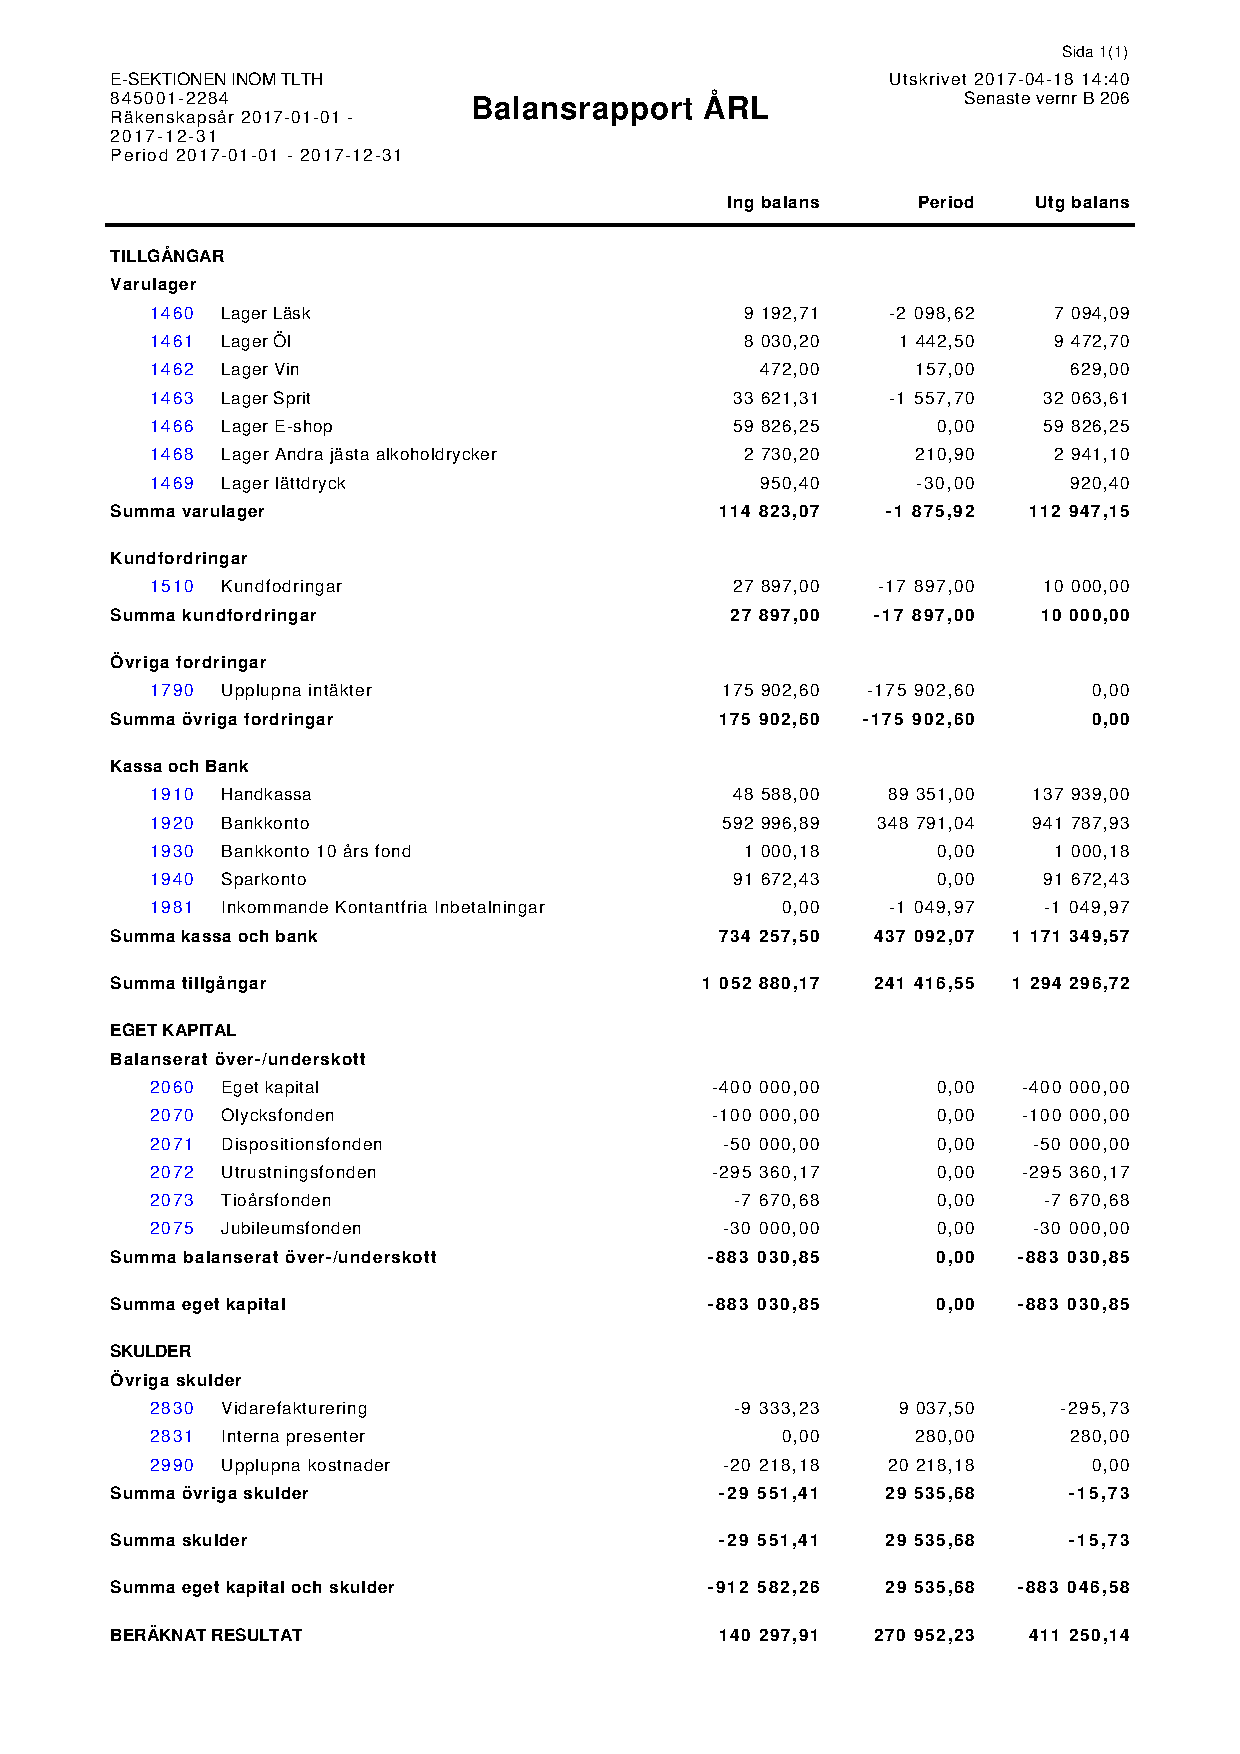
\includepdf[pages=1]{../_res/balansrapport.pdf}
\end{comment}
\subfile{../_other/uttag}
\newpage
\begin{supersection}{Beslutsuppföljningar}{}
    \subsection{Överblick}
    \begin{busek}
        \beslutsek{HT/16}{Fanbärare behöver längre påle}{Emil Harvig}{}{VT/17}
        \beslutsek{HT/16}{Införandet av arbetskläder för utlåning till funktionärer}{Martin Gemborn Nilsson}{}{VT/17}
        \beslutsek{HT/16}{Inköp av ny huvudswitch}{Erik Månsson}{}{VT/17}
        \beslutsek{HT/16}{Inköp av nya datorer}{Erik Månsson}{}{VT/17}
        \beslutsek{HT/16}{Uppdatering av övervakningspolicyn}{Styrelsen}{}{VT/17}
        \beslutsek{VT/16}{Renovering och ombyggnad av HK och BD}{Styrelsen 2016}{Rusta upp HK och BD och bland annat flytta väggen mellan rummen till en kostnad av maximalt \SI{30000}{kr}}{VT/17}
        \beslutsek{VT/16}{Uppfräschning av gamla arkivet}{Styrelsen 2016}{Rusta upp gamla arkivet med bland annat nya inventarier till en kostnad av maximalt \SI{10000}{kr}}{VT/17}
    \end{busek}
    \newpage

    \subfile{../besuppf/fanb}
    %\subfile{../besuppf/arbkl}
    \subfile{../besuppf/switch}
    \subfile{../besuppf/datorer}
    \subfile{../besuppf/overvakn}
    \subfile{../besuppf/hkbd}
    \subfile{../besuppf/arkivet}
\end{supersection}

\begin{utskottsrapporter}
%    \subfile{../utskottsrapporter/cm}
    \subfile{../utskottsrapporter/e6}
    \subfile{../utskottsrapporter/enu}
%    \subfile{../utskottsrapporter/fvu}
%    \subfile{../utskottsrapporter/infu}
%    \subfile{../utskottsrapporter/km}
    \subfile{../utskottsrapporter/noju}
%    \subfile{../utskottsrapporter/nollu}
    \subfile{../utskottsrapporter/sre}
    \subfile{../utskottsrapporter/styret}
%    \subfile{../utskottsrapporter/vb}
\end{utskottsrapporter}

\begin{comment} %TODO
\begin{supersection}{Verksamhetsplaner}{}
    \subfile{../verksplaner/2016}
    \subfile{../verksplaner/2017}
\end{supersection}

\begin{supersection}{Uppföljningar av verksamhetsplaner}{}
    %\subfile{../verksplanuppfar/2016-vt}
    %\subfile{../verksplanuppfar/2016-ht}
    \subfile{../verksplanuppfar/2017-vt-avg}
    \subfile{../verksplanuppfar/2017-vt-nuv}
\end{supersection}

\begin{berattelser}
    \subfile{../berattelser/styret}
    \subfile{../berattelser/cm}
    \subfile{../berattelser/e6}
    \subfile{../berattelser/enu}
    \subfile{../berattelser/fvu}
    \subfile{../berattelser/infu}
    \subfile{../berattelser/km}
    \subfile{../berattelser/noju}
    \subfile{../berattelser/nollu}
    \subfile{../berattelser/sre}
    \subfile{../berattelser/vb}
\end{berattelser}

\begin{motioner}
    \subfile{../motioner/x}
    \subfile{../motionssvar/x}
\end{motioner}

\begin{propositioner}
    \subfile{../propositioner/}
    \subfile{../propositioner/}
    \subfile{../propositioner/}
    \subfile{../propositioner/}
\end{propositioner}

\begin{supersection}{Halvårsbokslut 2016}{}
    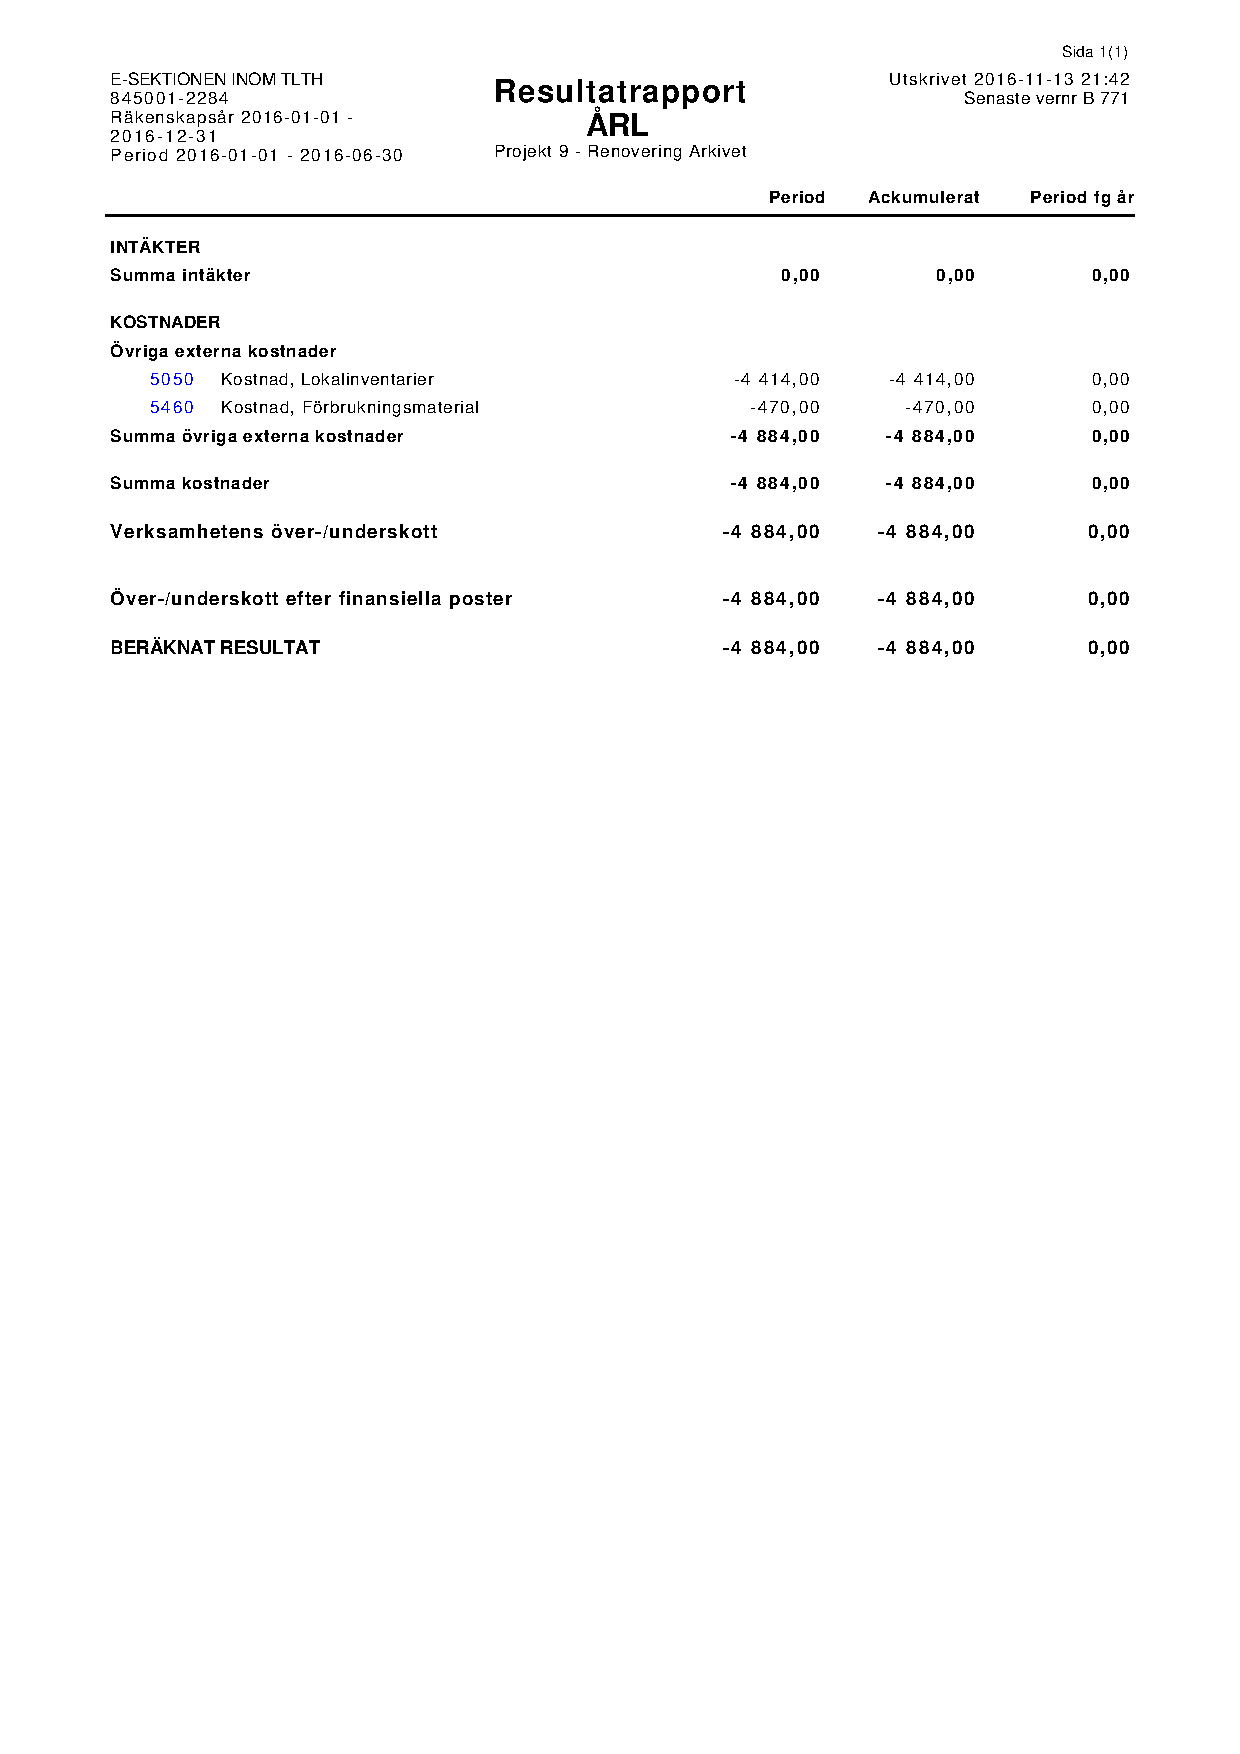
\includepdf[pages=-]{../_res/bokslut/arkivet.pdf}
    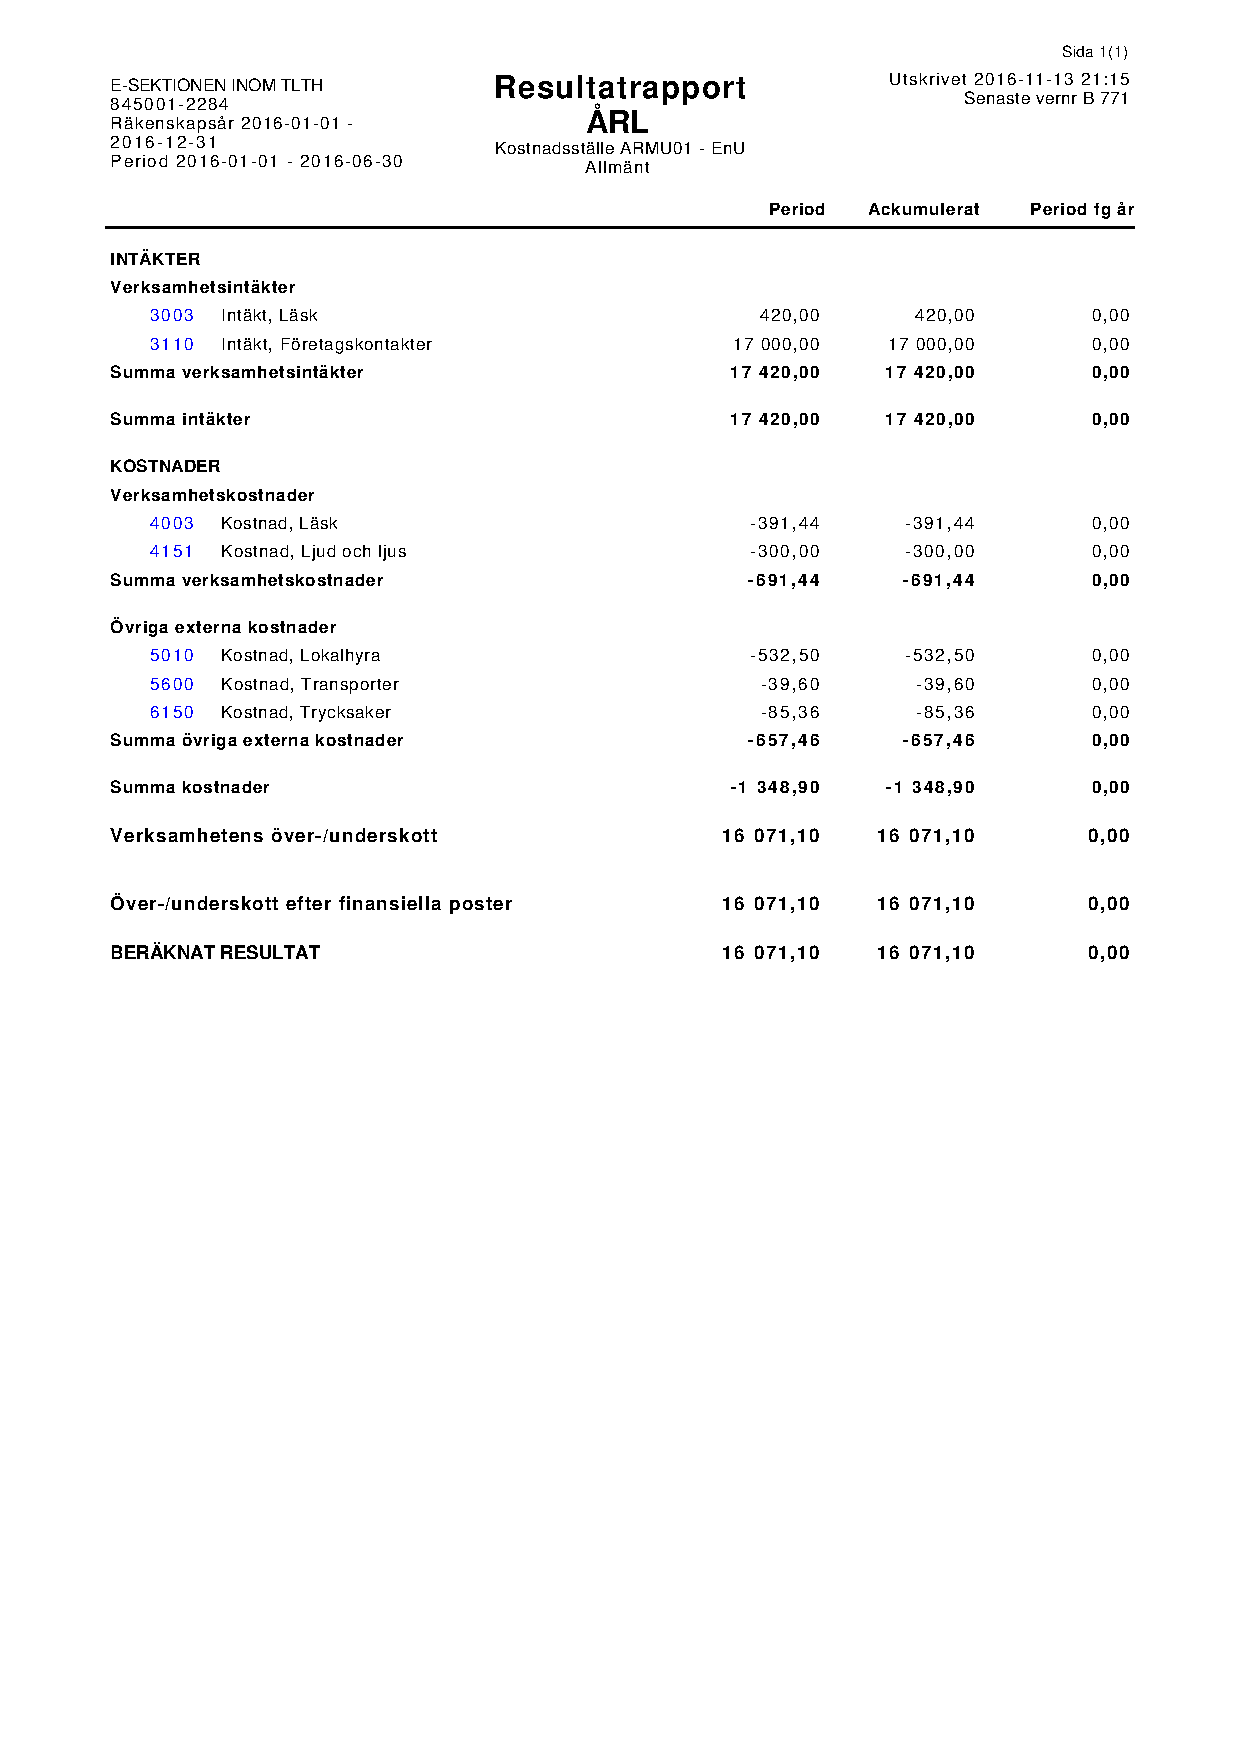
\includepdf[pages=-]{../_res/bokslut/armu01.pdf}
    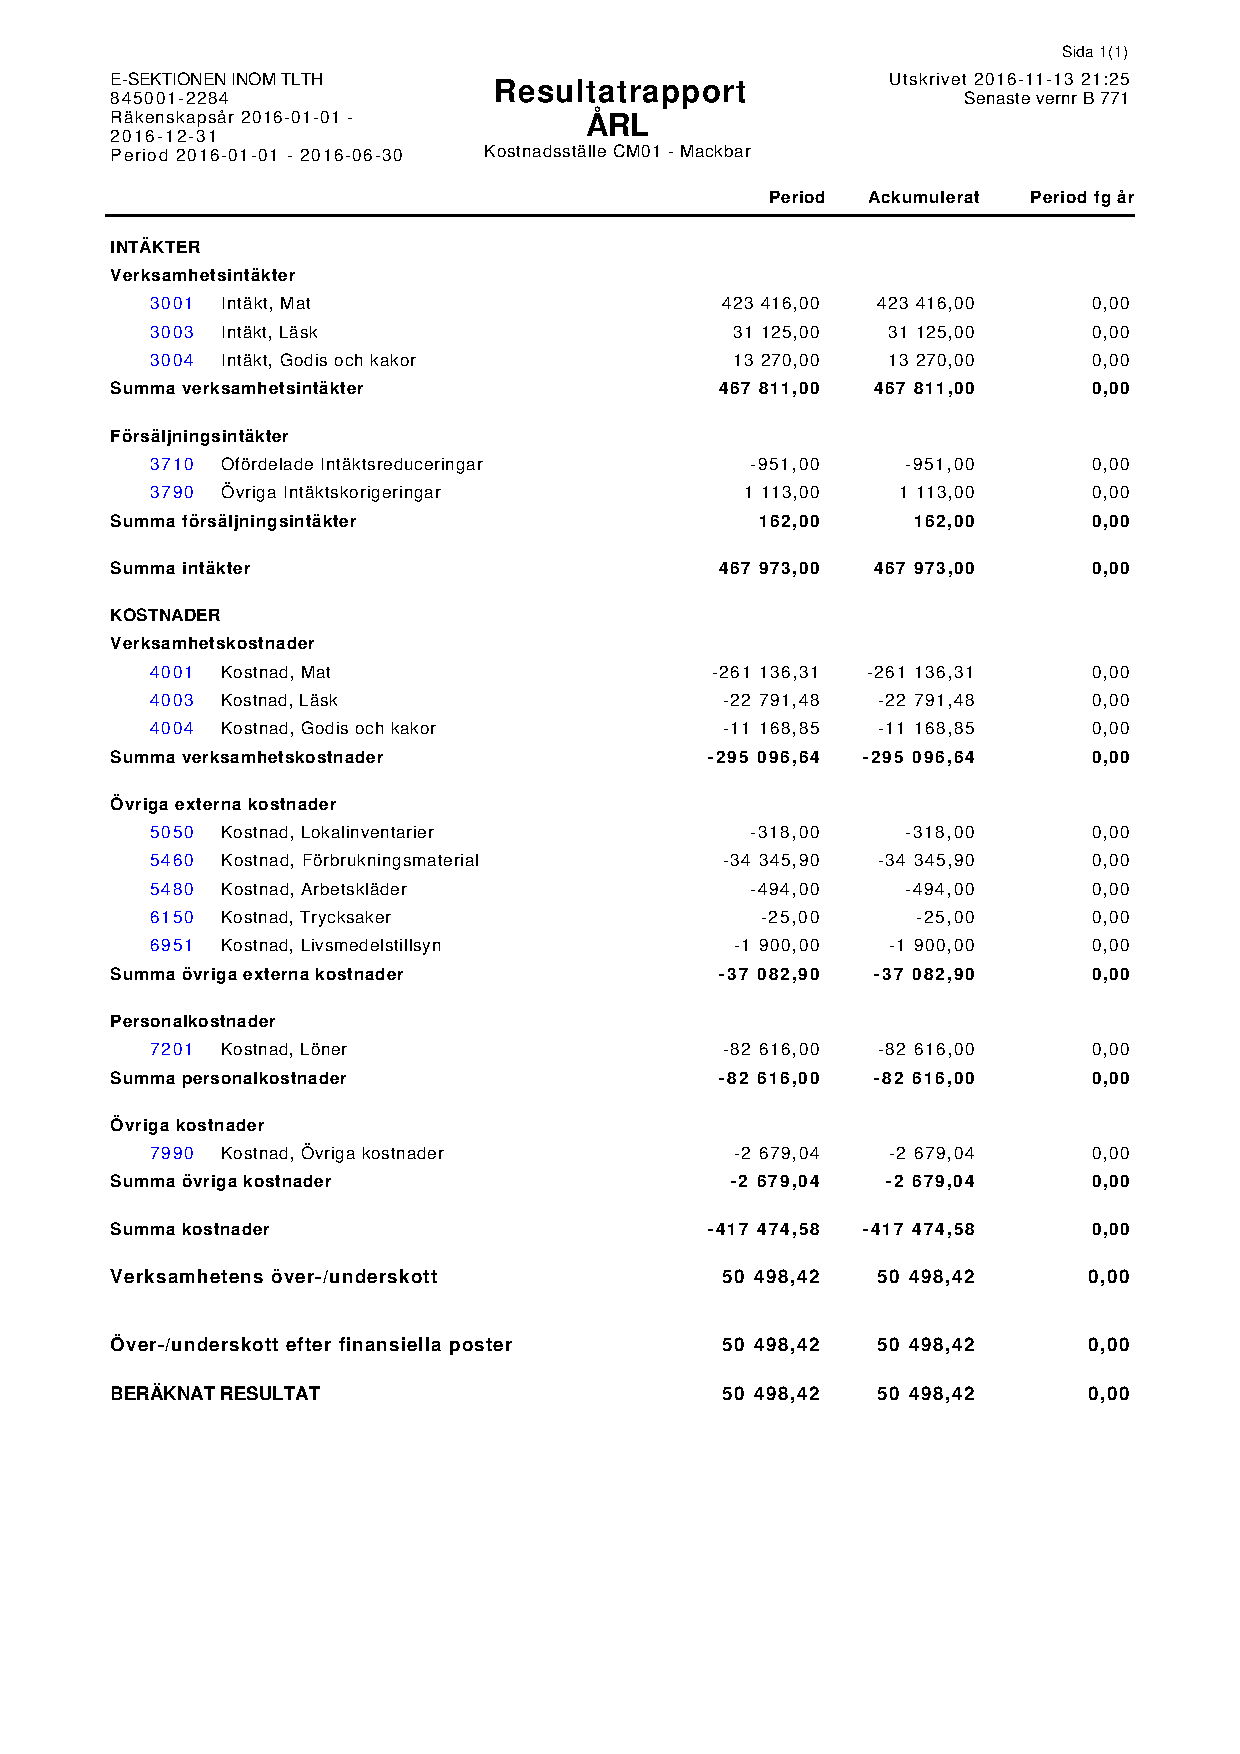
\includepdf[pages=-]{../_res/bokslut/cm01.pdf}
    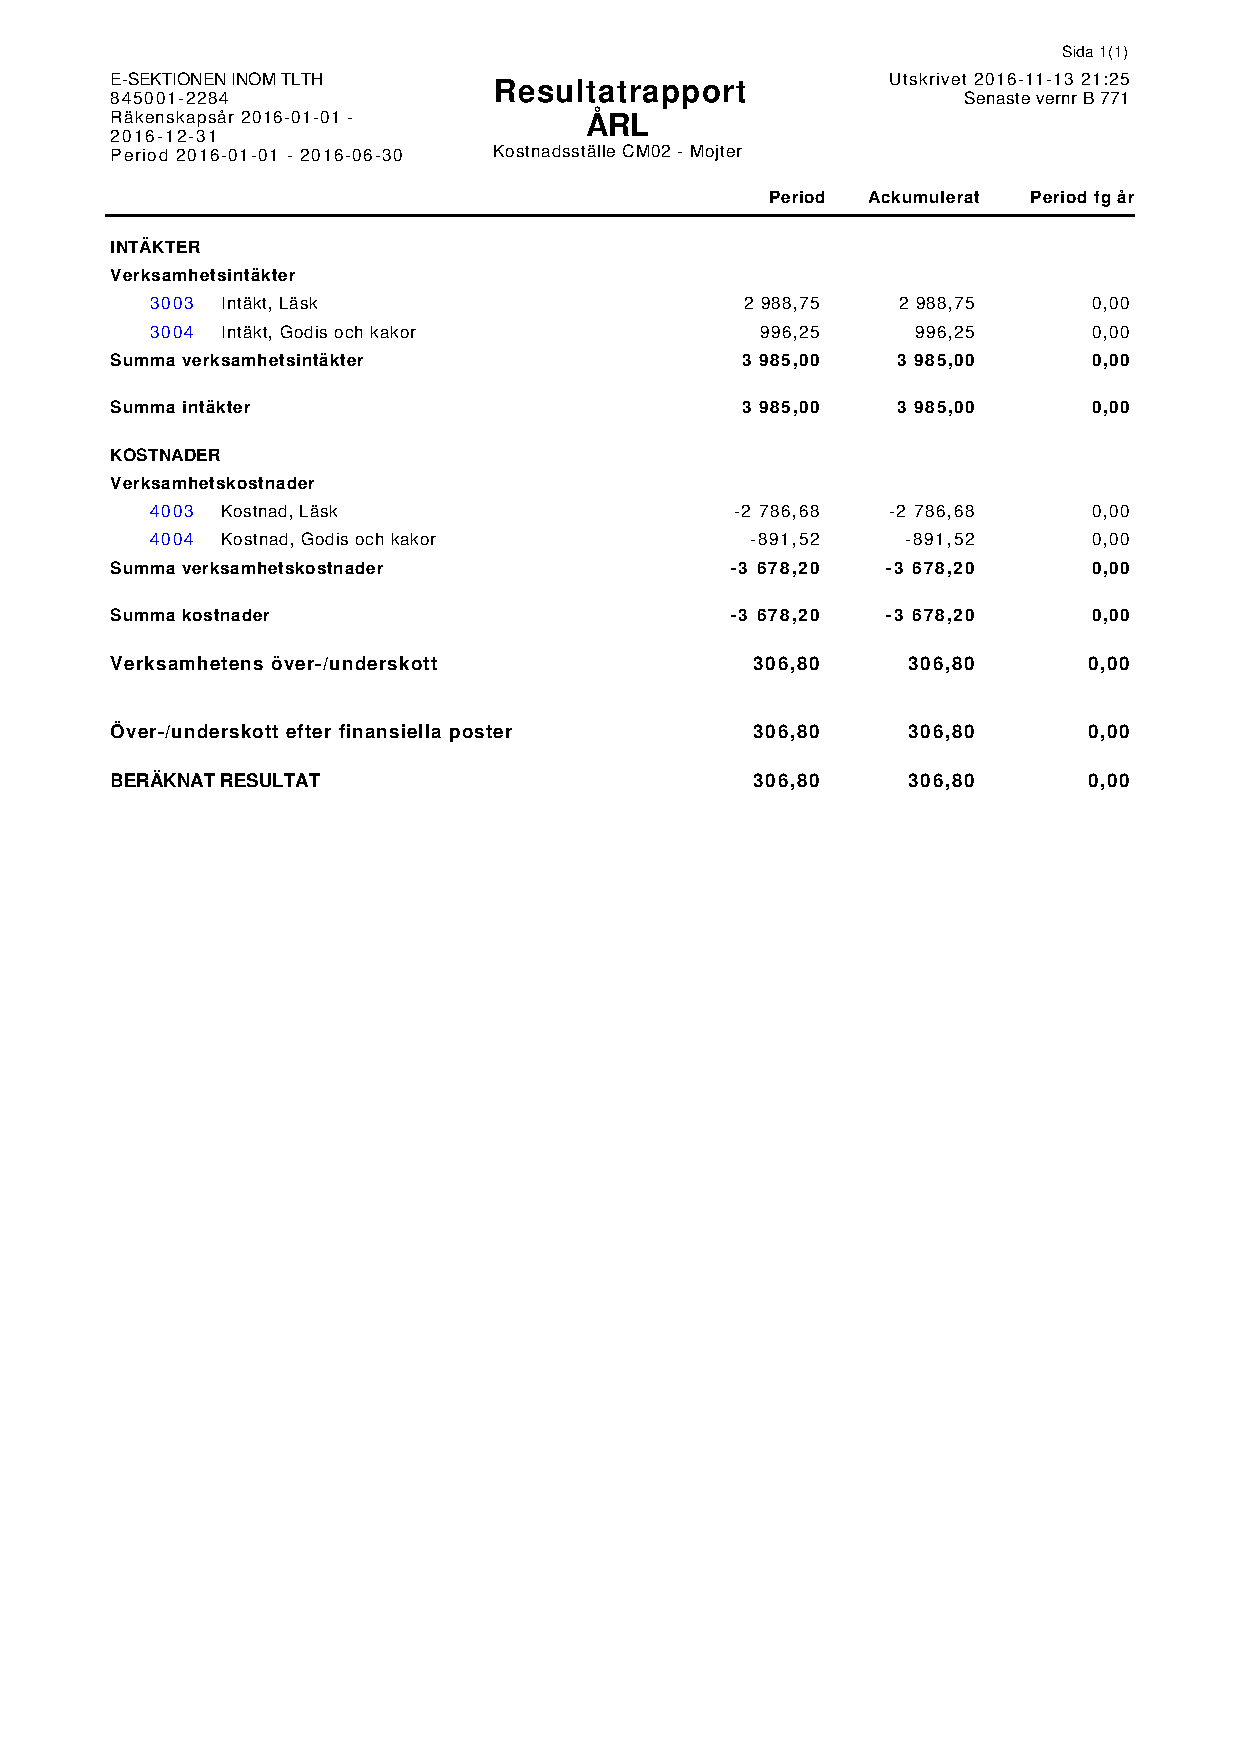
\includepdf[pages=-]{../_res/bokslut/cm02.pdf}
    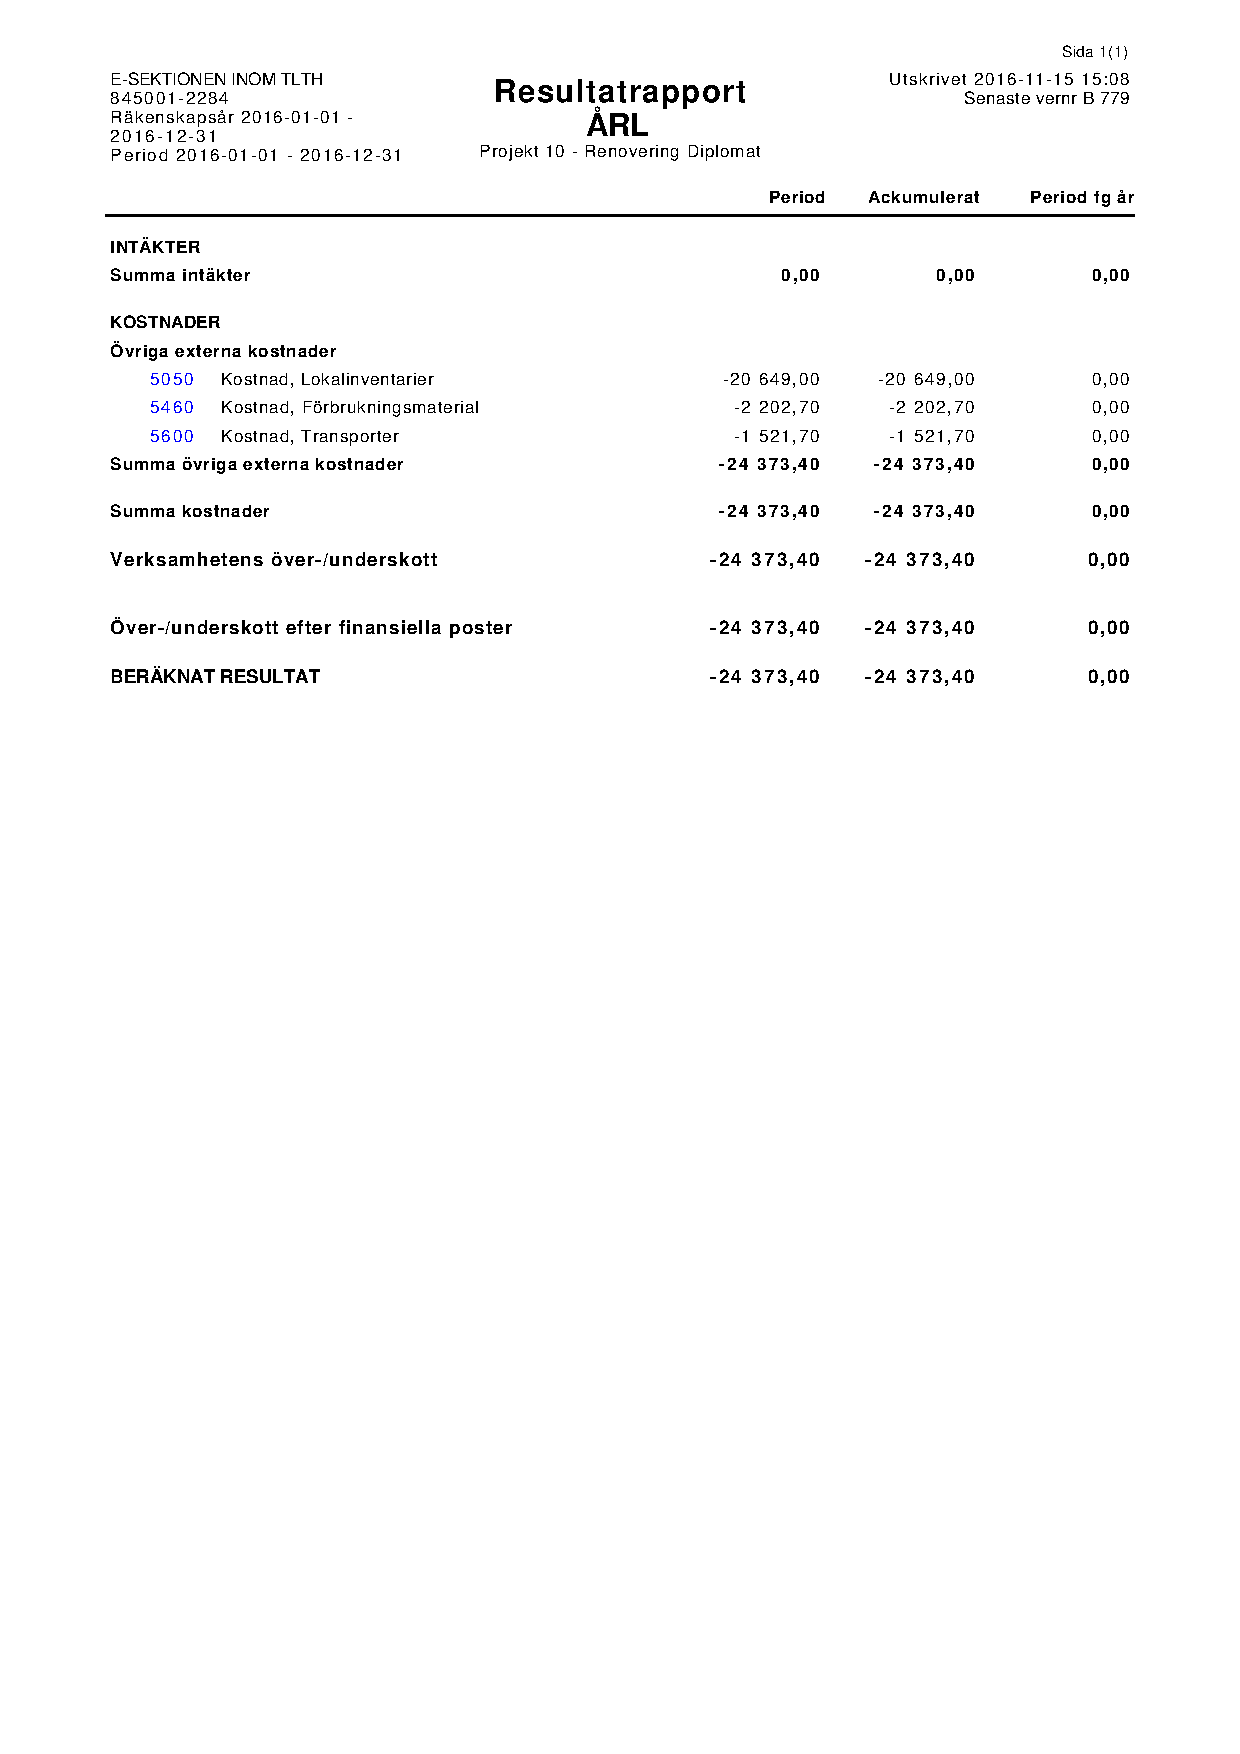
\includepdf[pages=-]{../_res/bokslut/diplomat.pdf}
    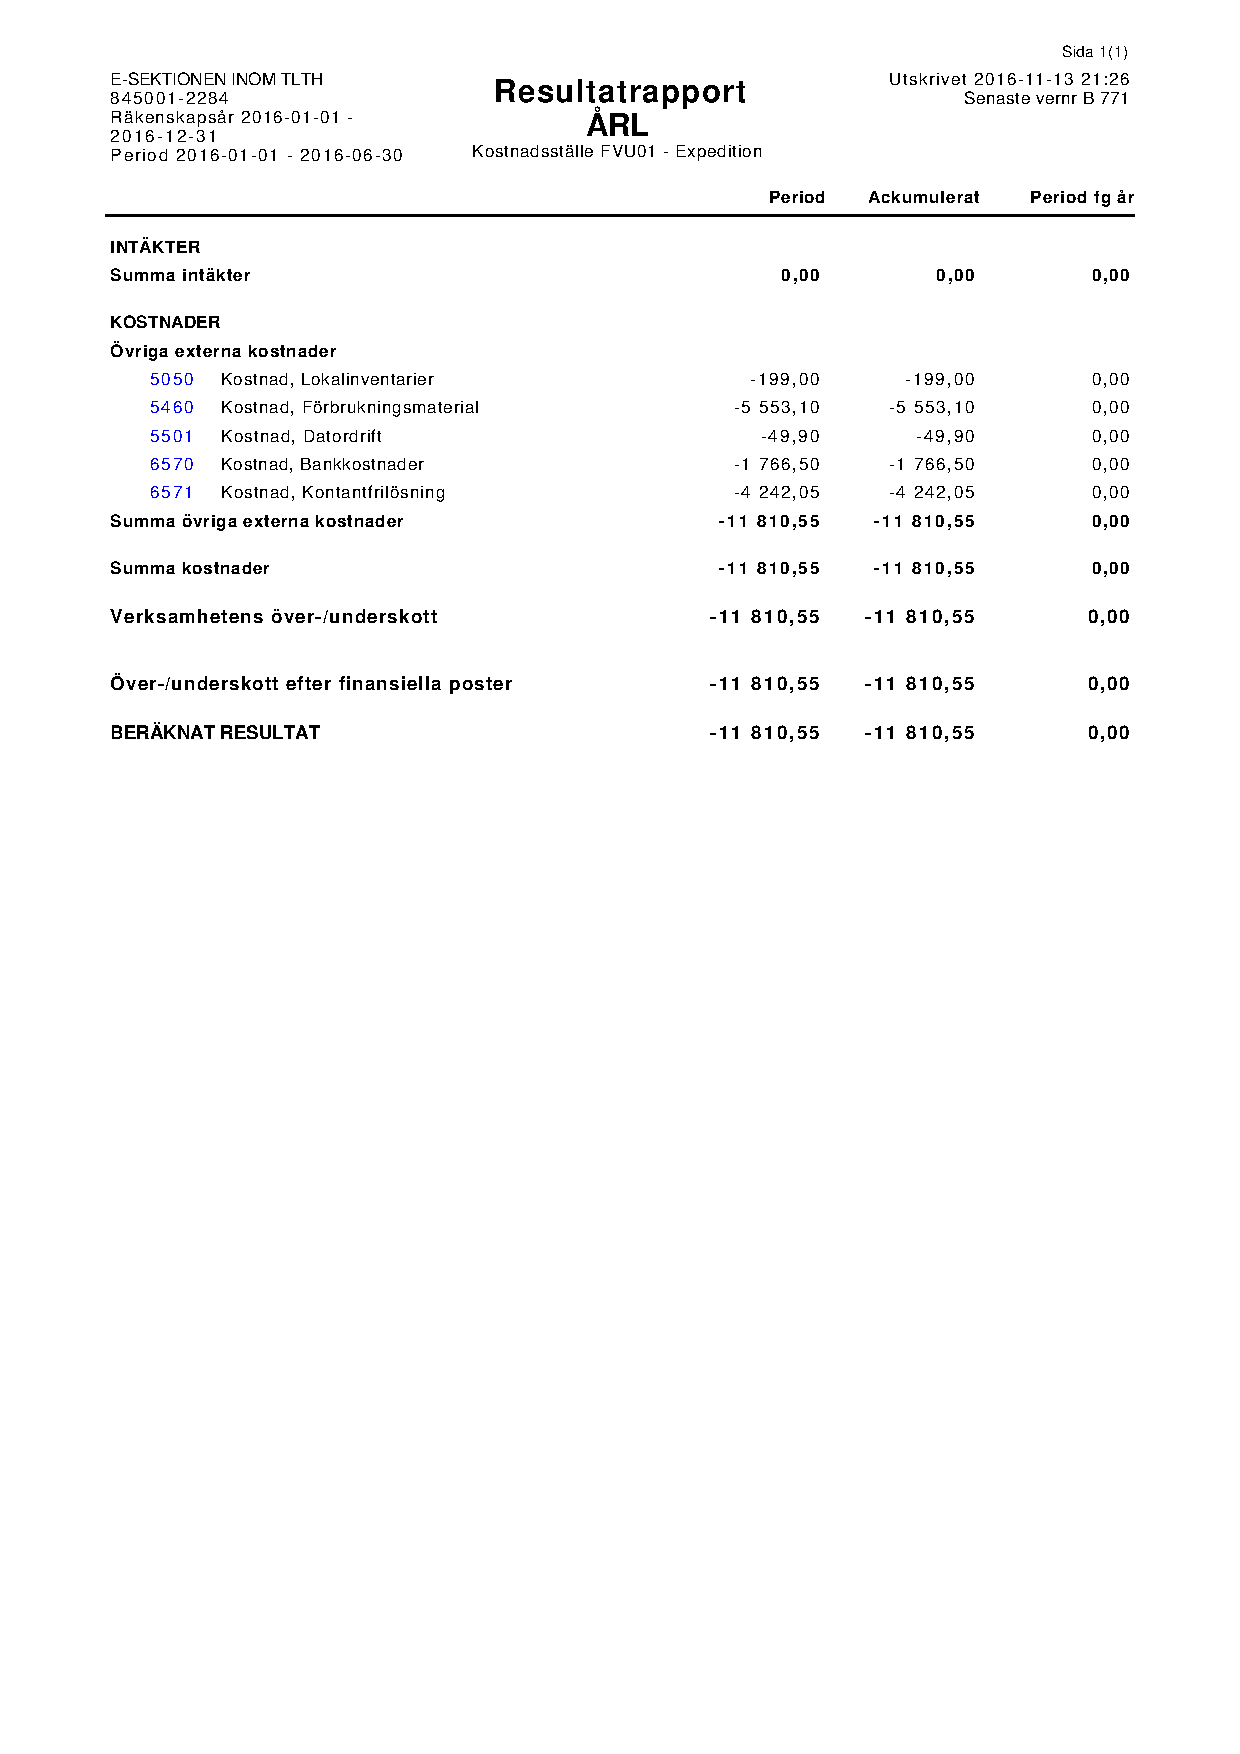
\includepdf[pages=-]{../_res/bokslut/fvu01.pdf}
    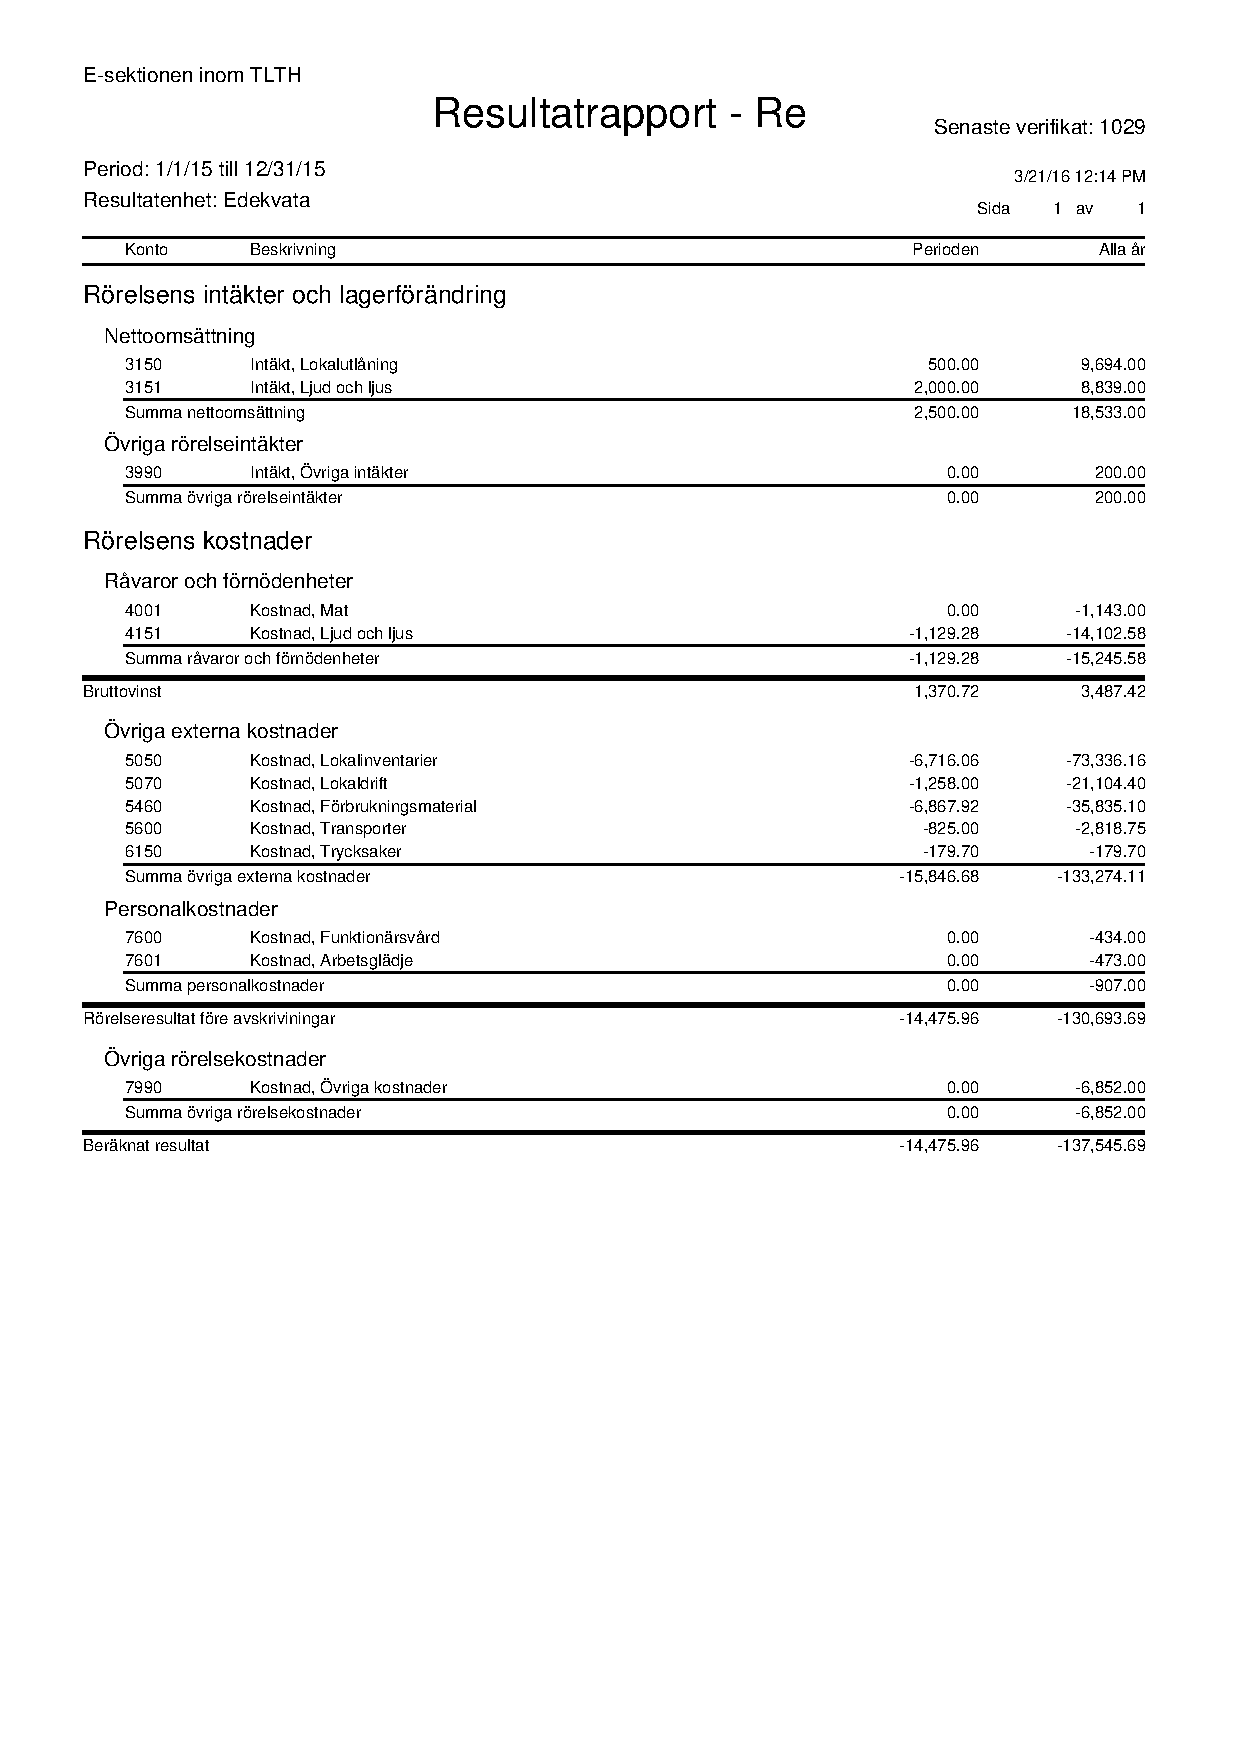
\includepdf[pages=-]{../_res/bokslut/fvu02.pdf}
    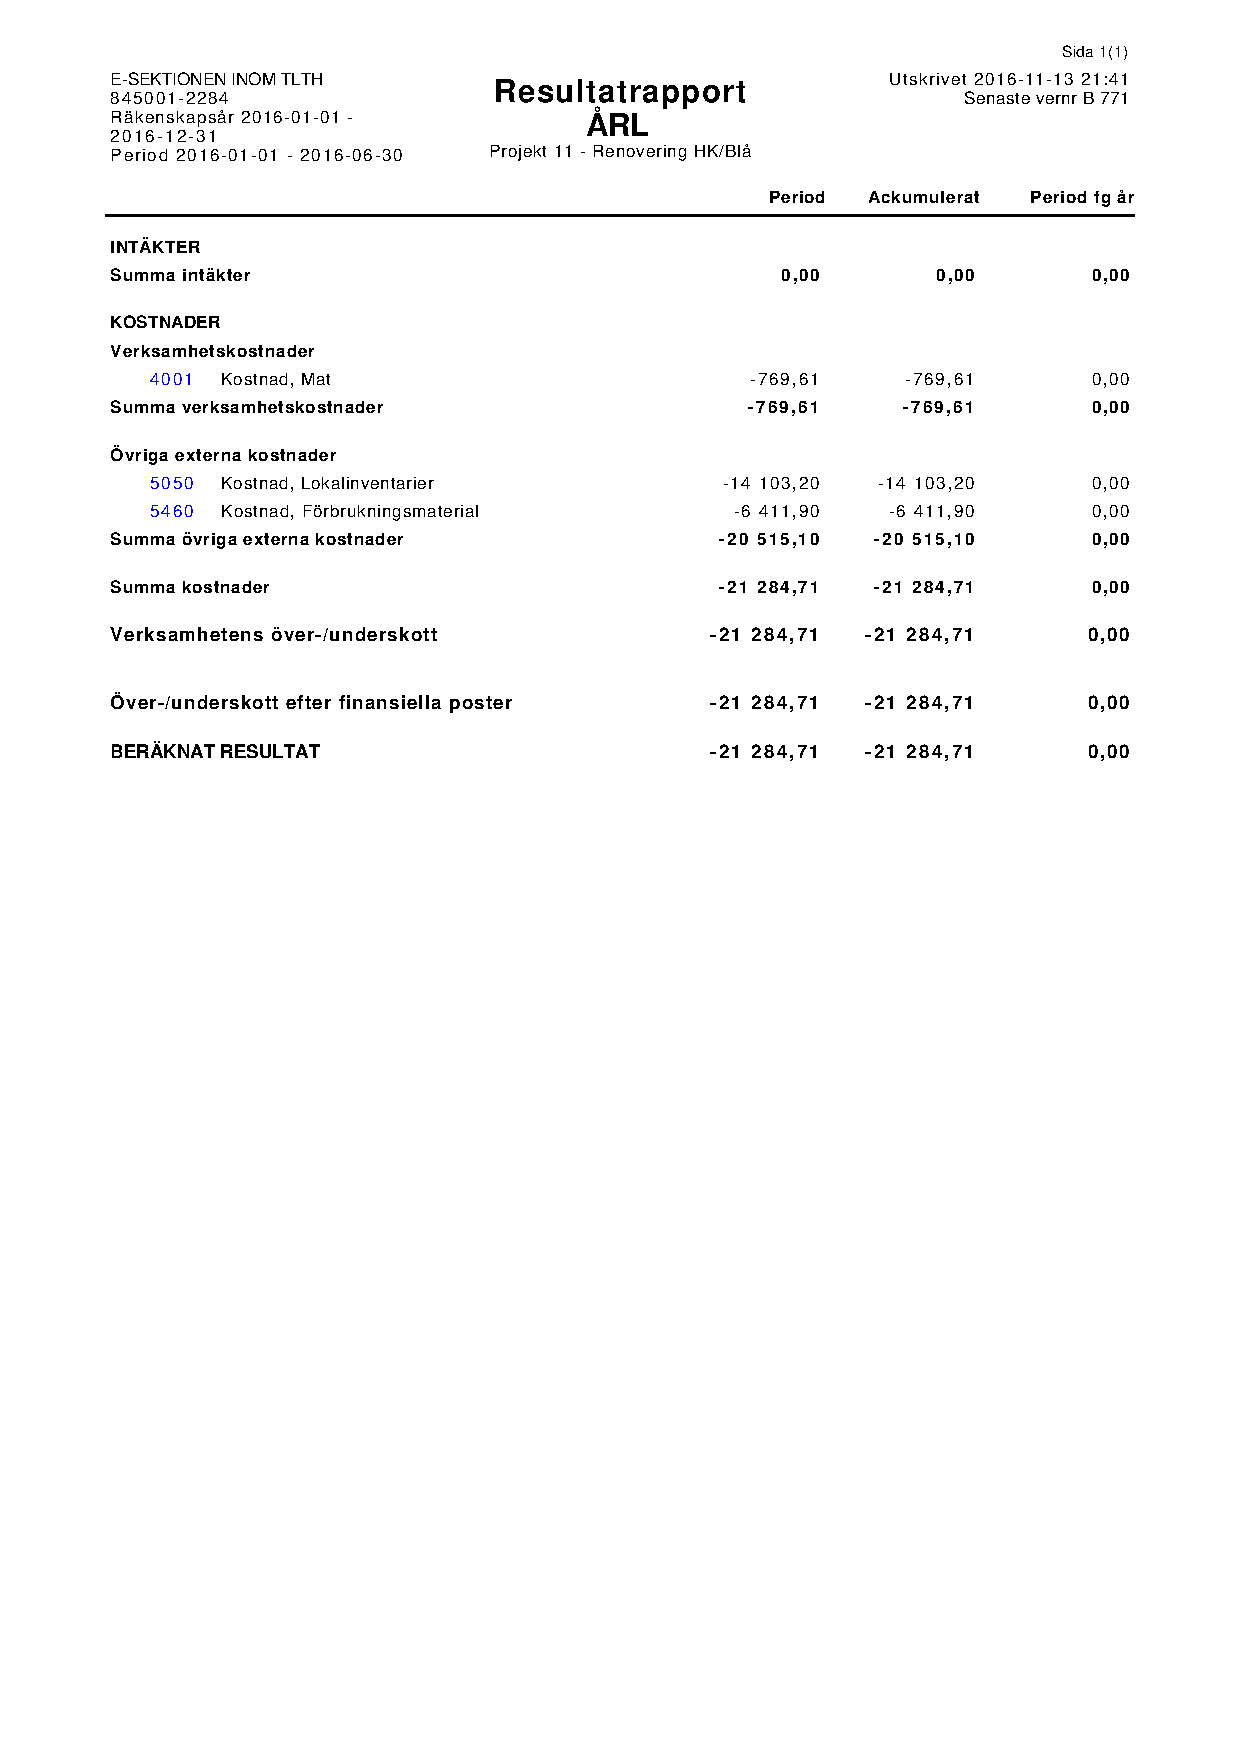
\includepdf[pages=-]{../_res/bokslut/hk.pdf}
    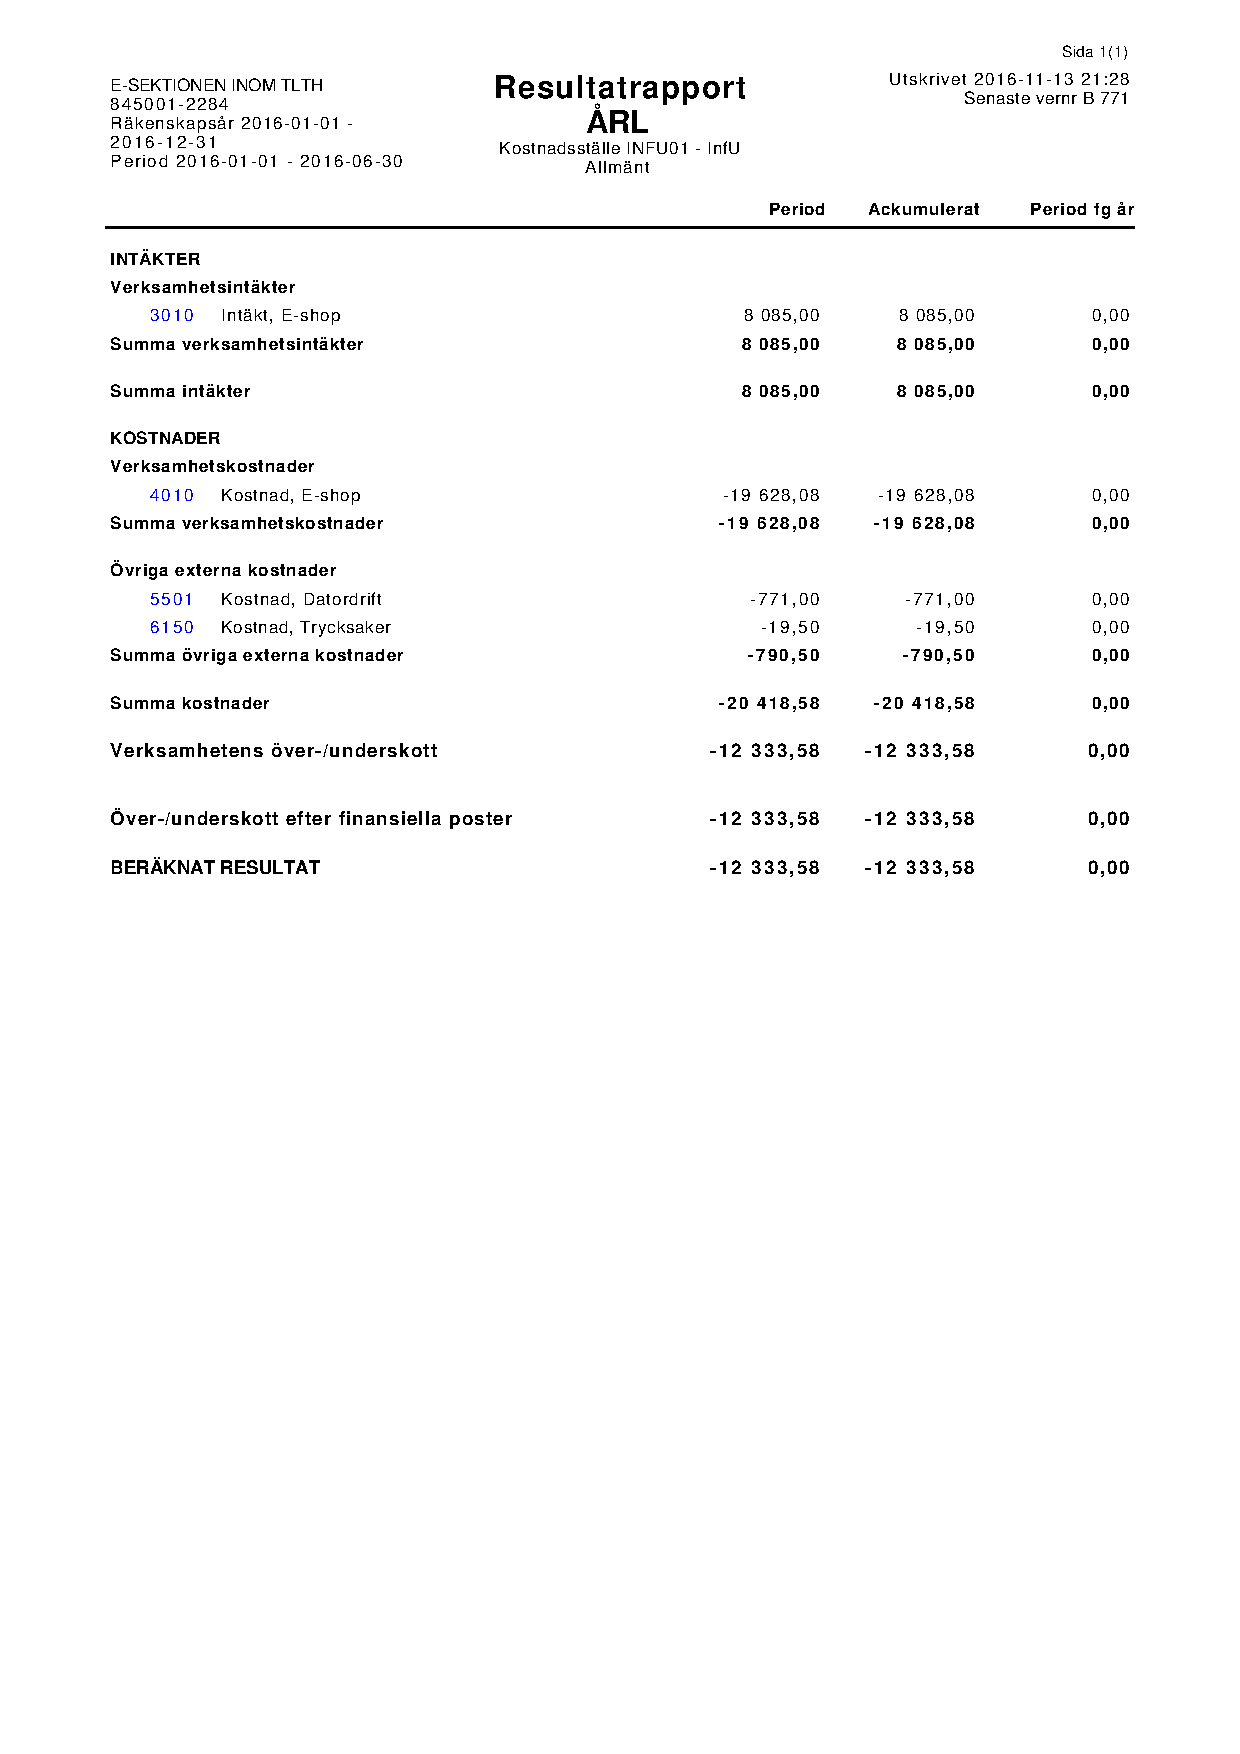
\includepdf[pages=-]{../_res/bokslut/infu01.pdf}
    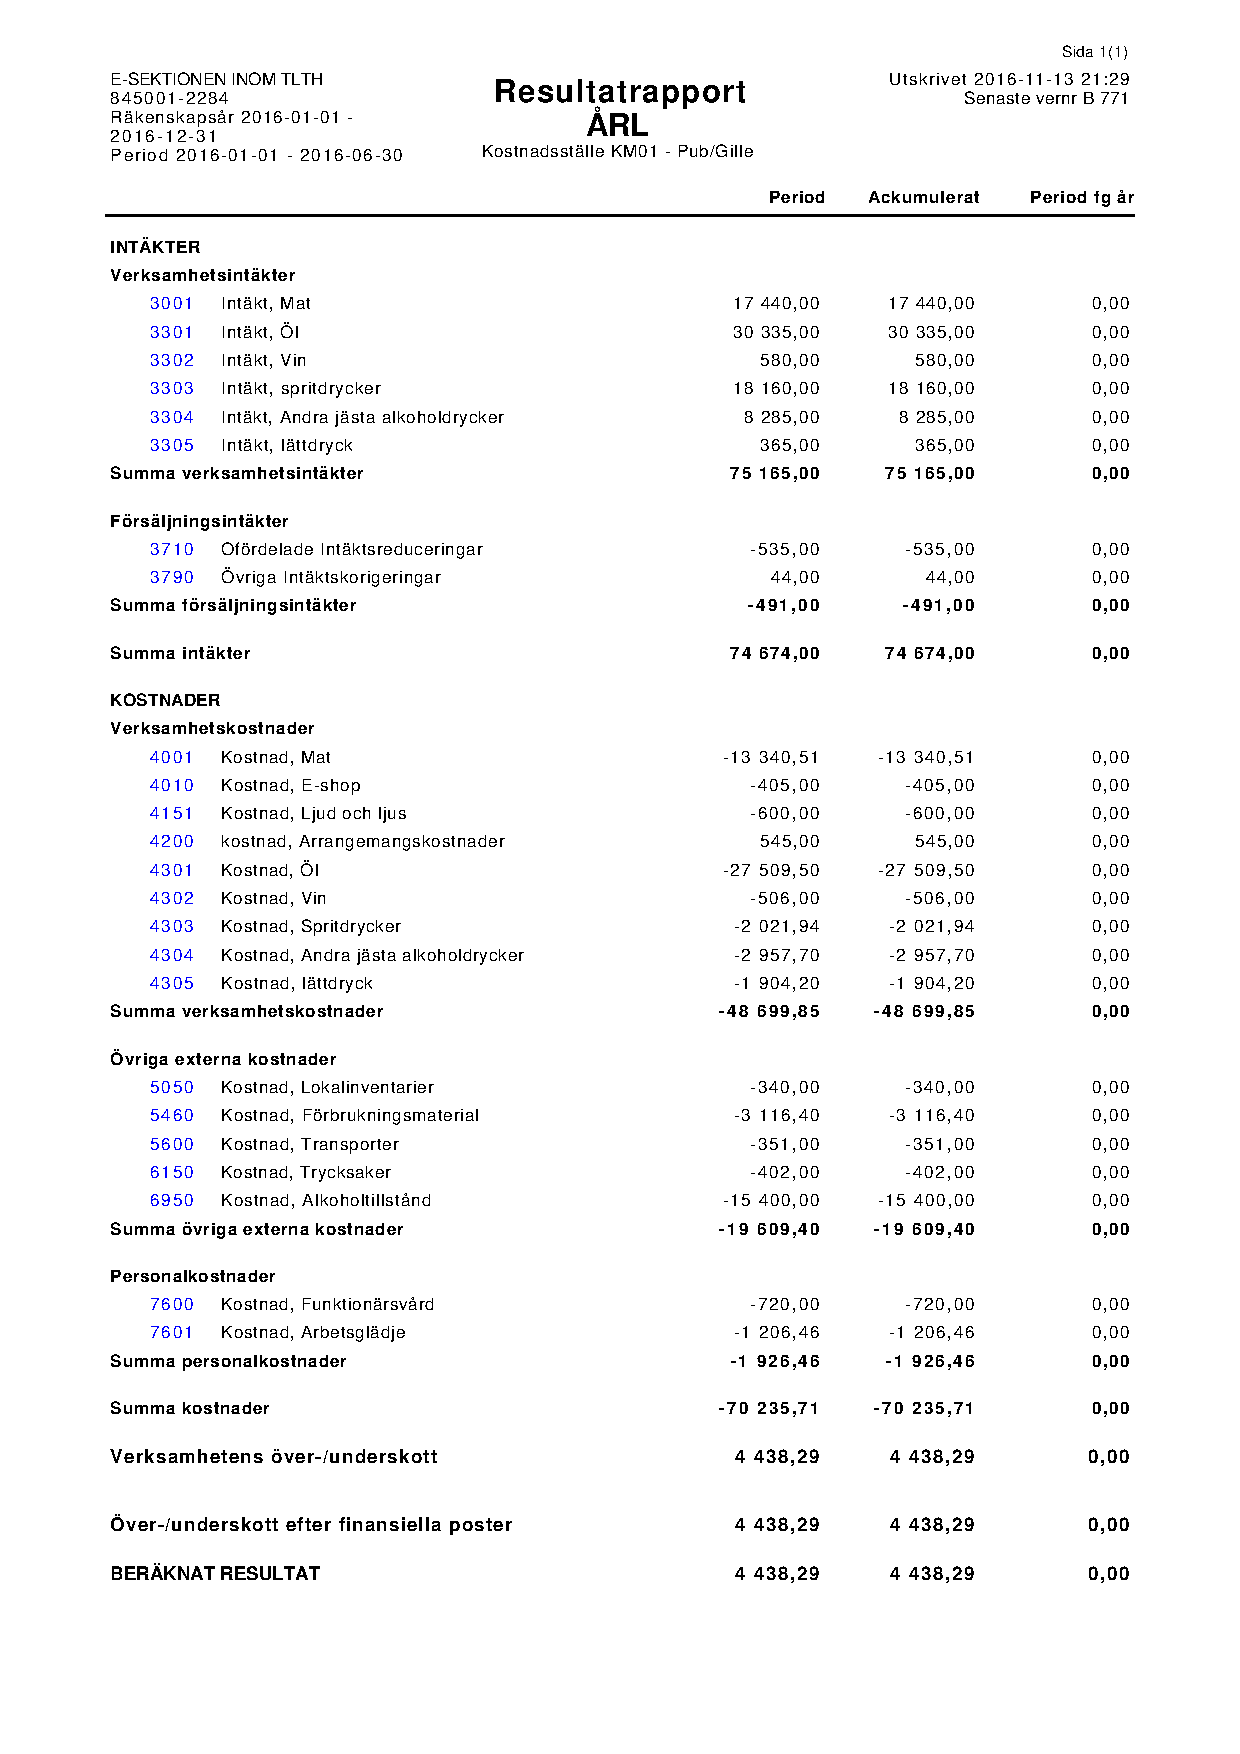
\includepdf[pages=-]{../_res/bokslut/km01.pdf}
    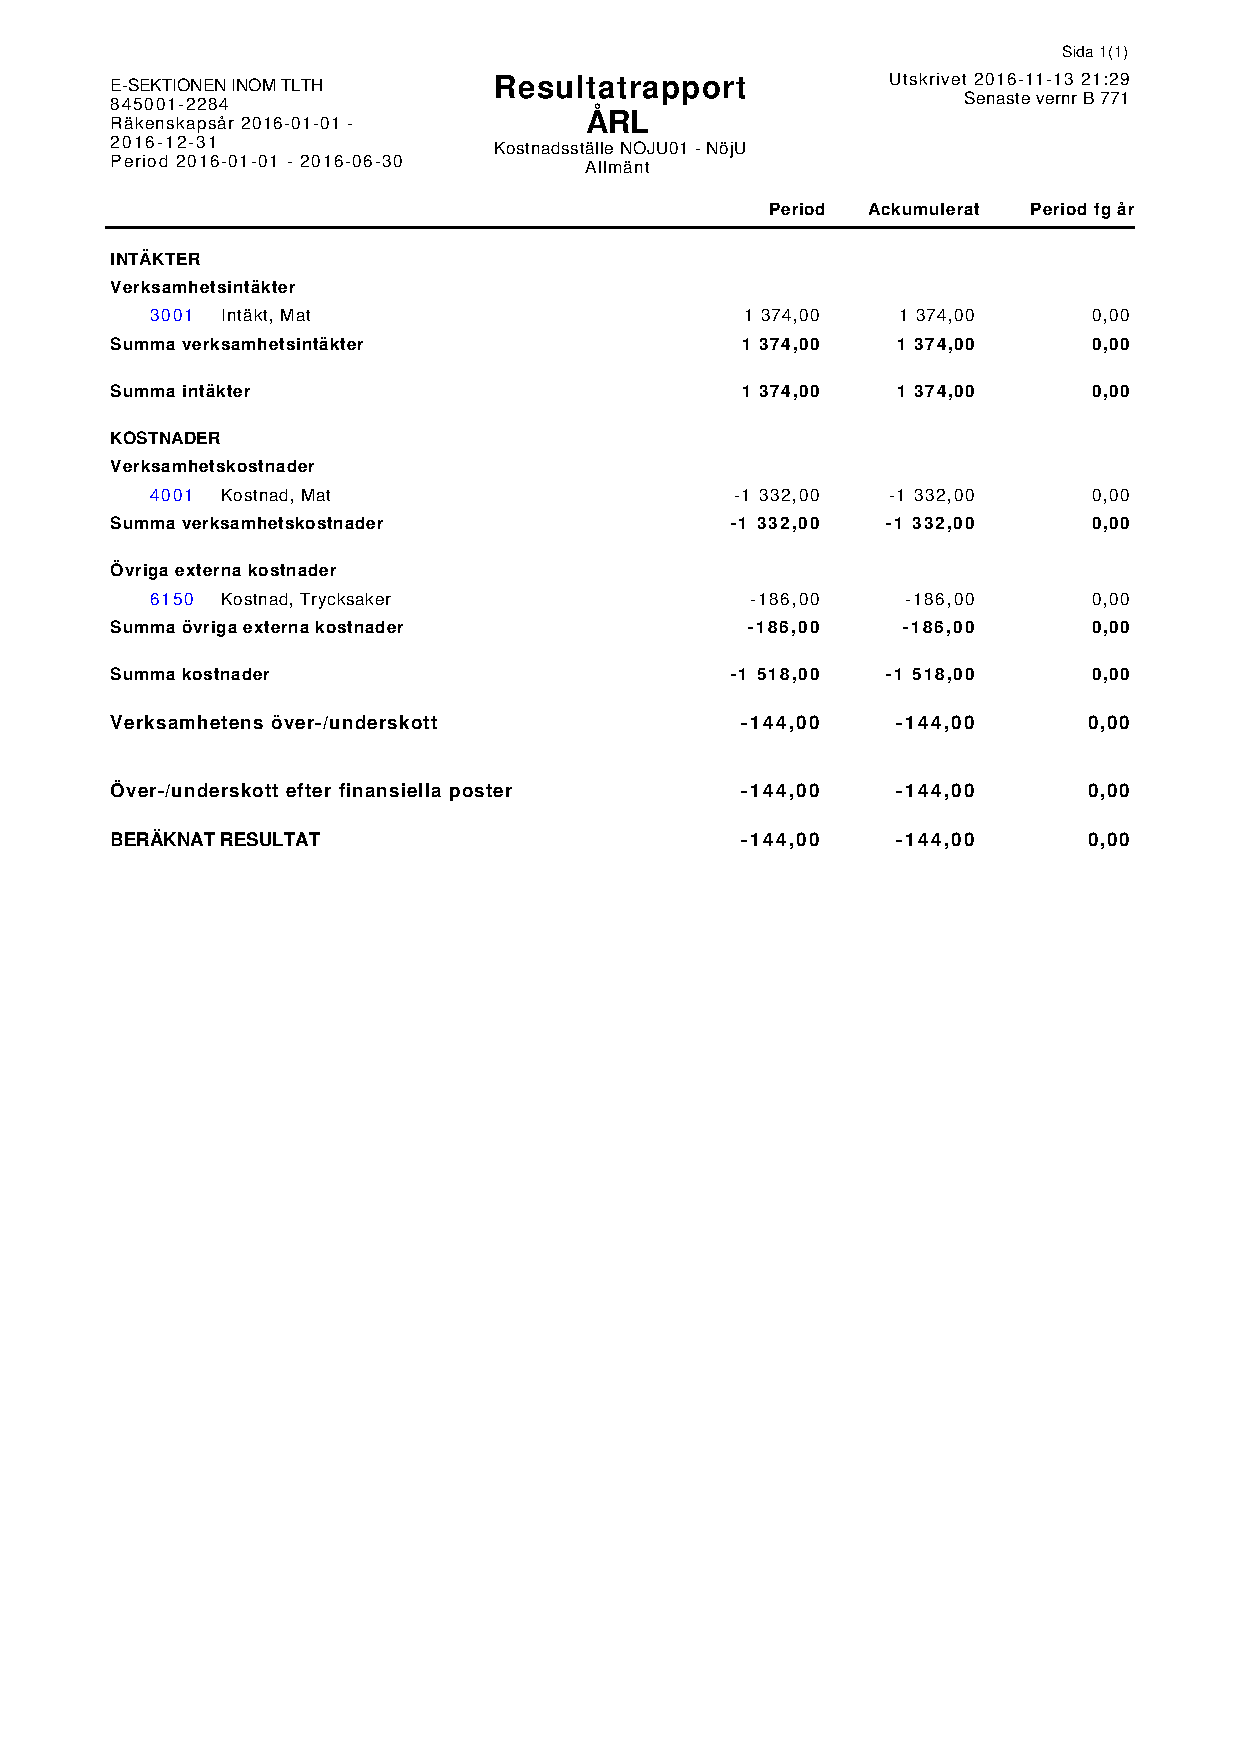
\includepdf[pages=-]{../_res/bokslut/noju01.pdf}
    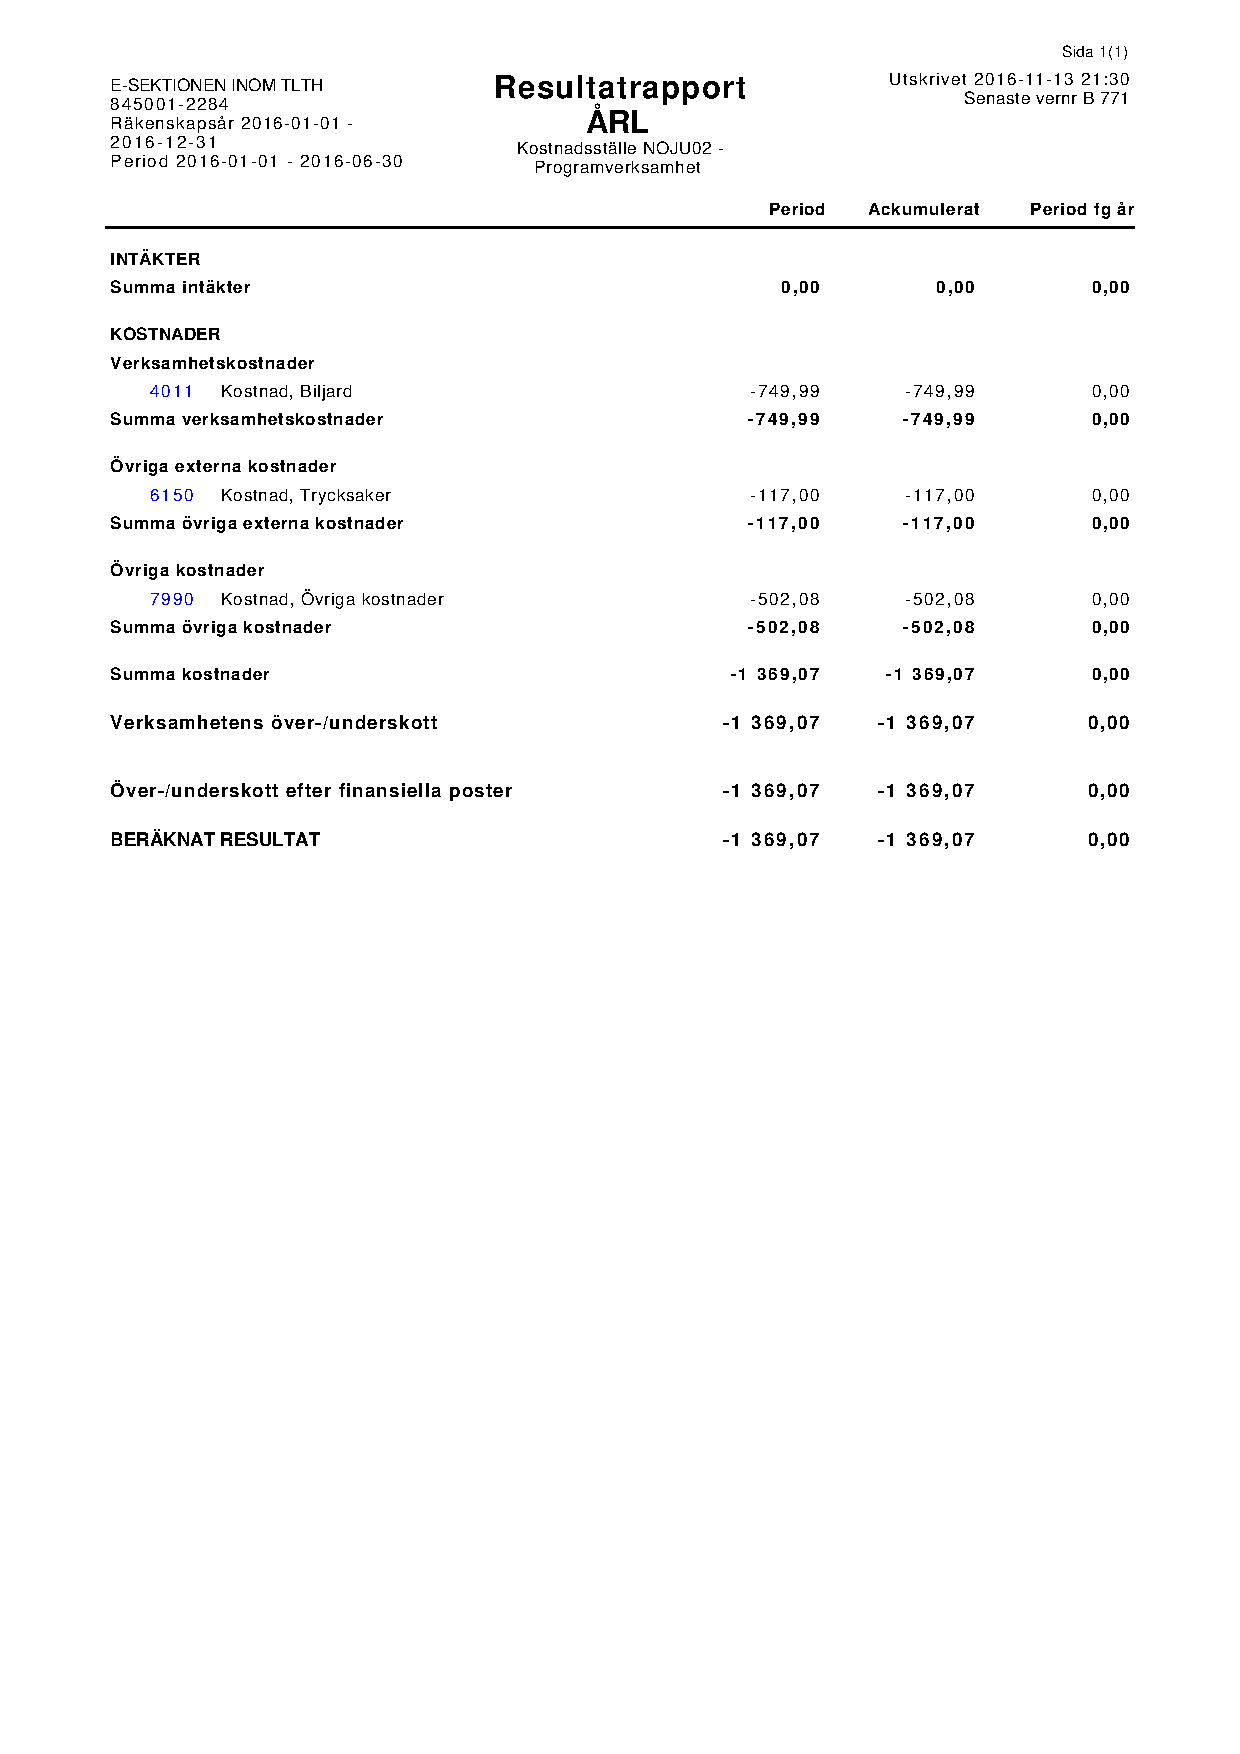
\includepdf[pages=-]{../_res/bokslut/noju02.pdf}
    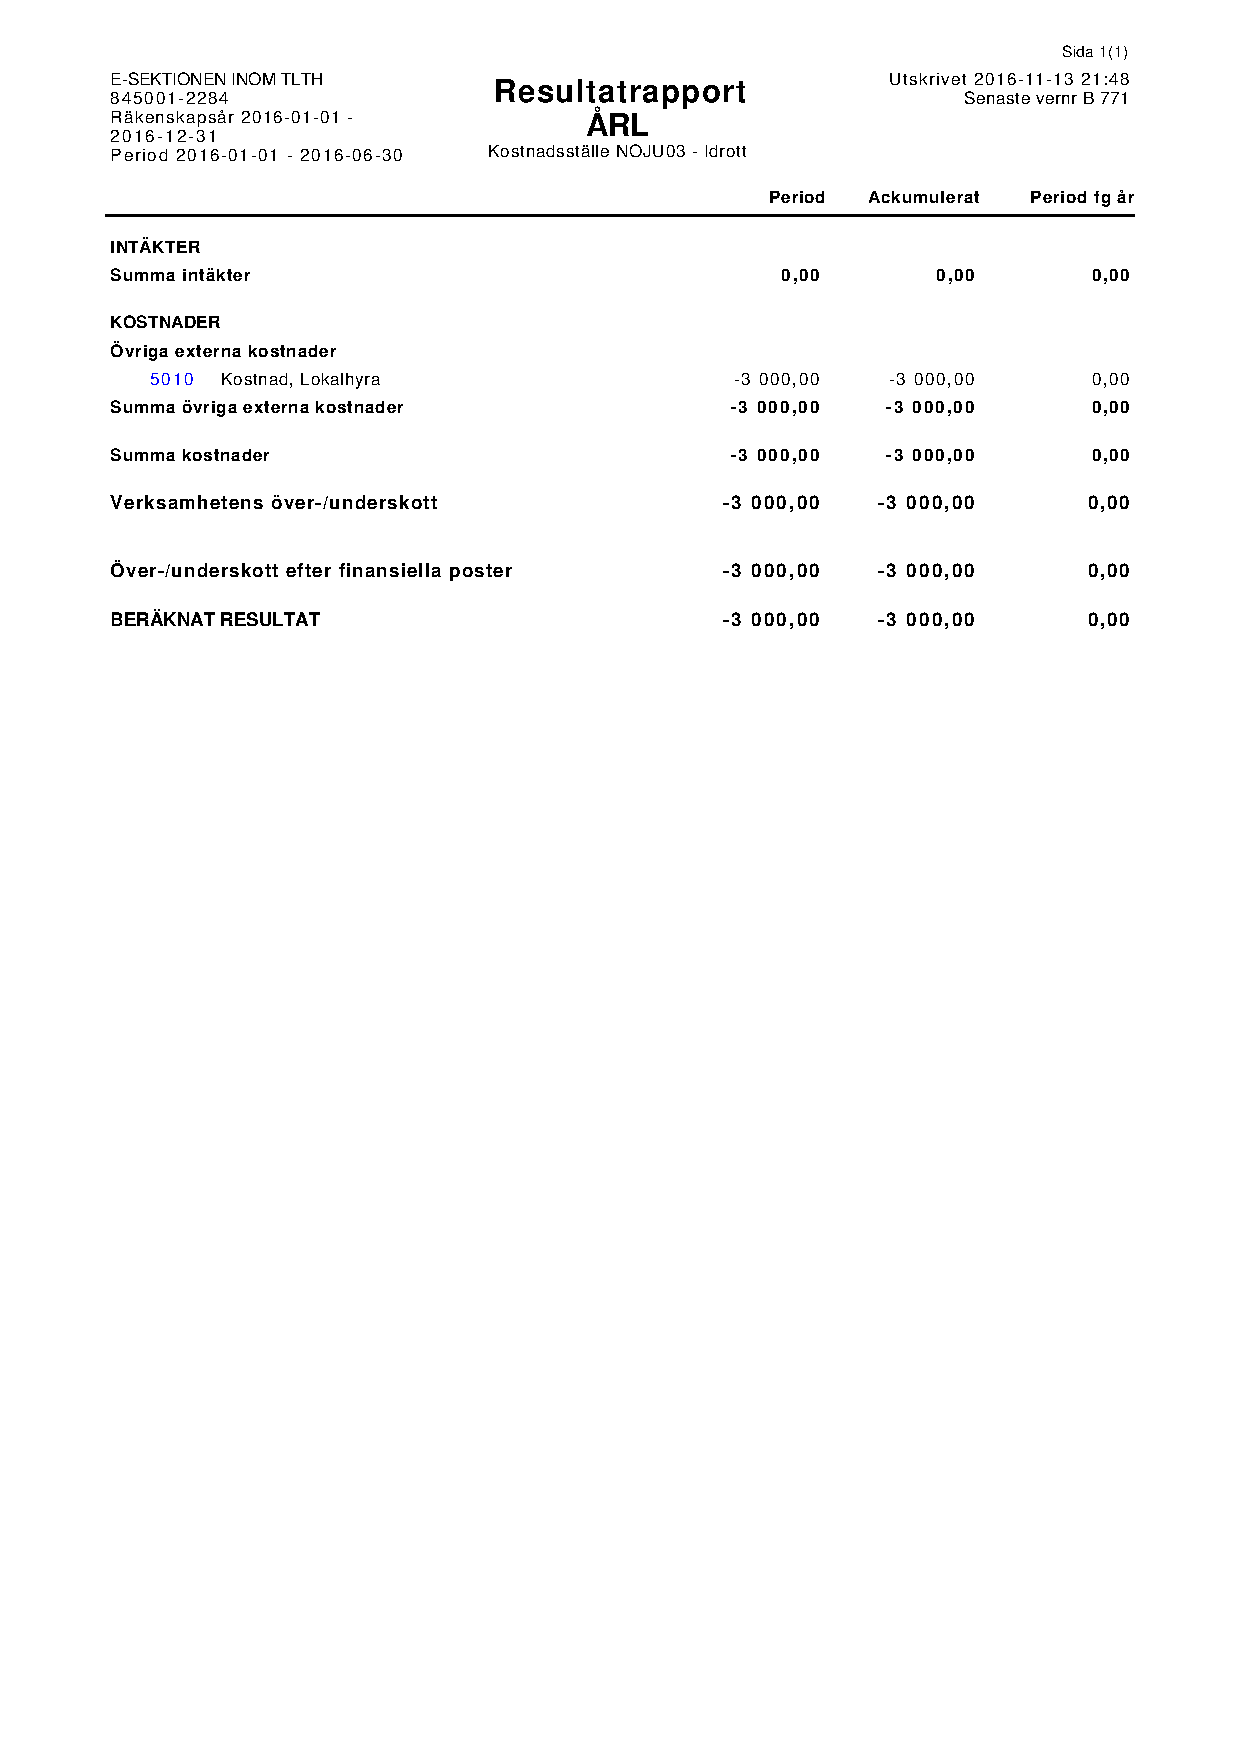
\includepdf[pages=-]{../_res/bokslut/noju03.pdf}
    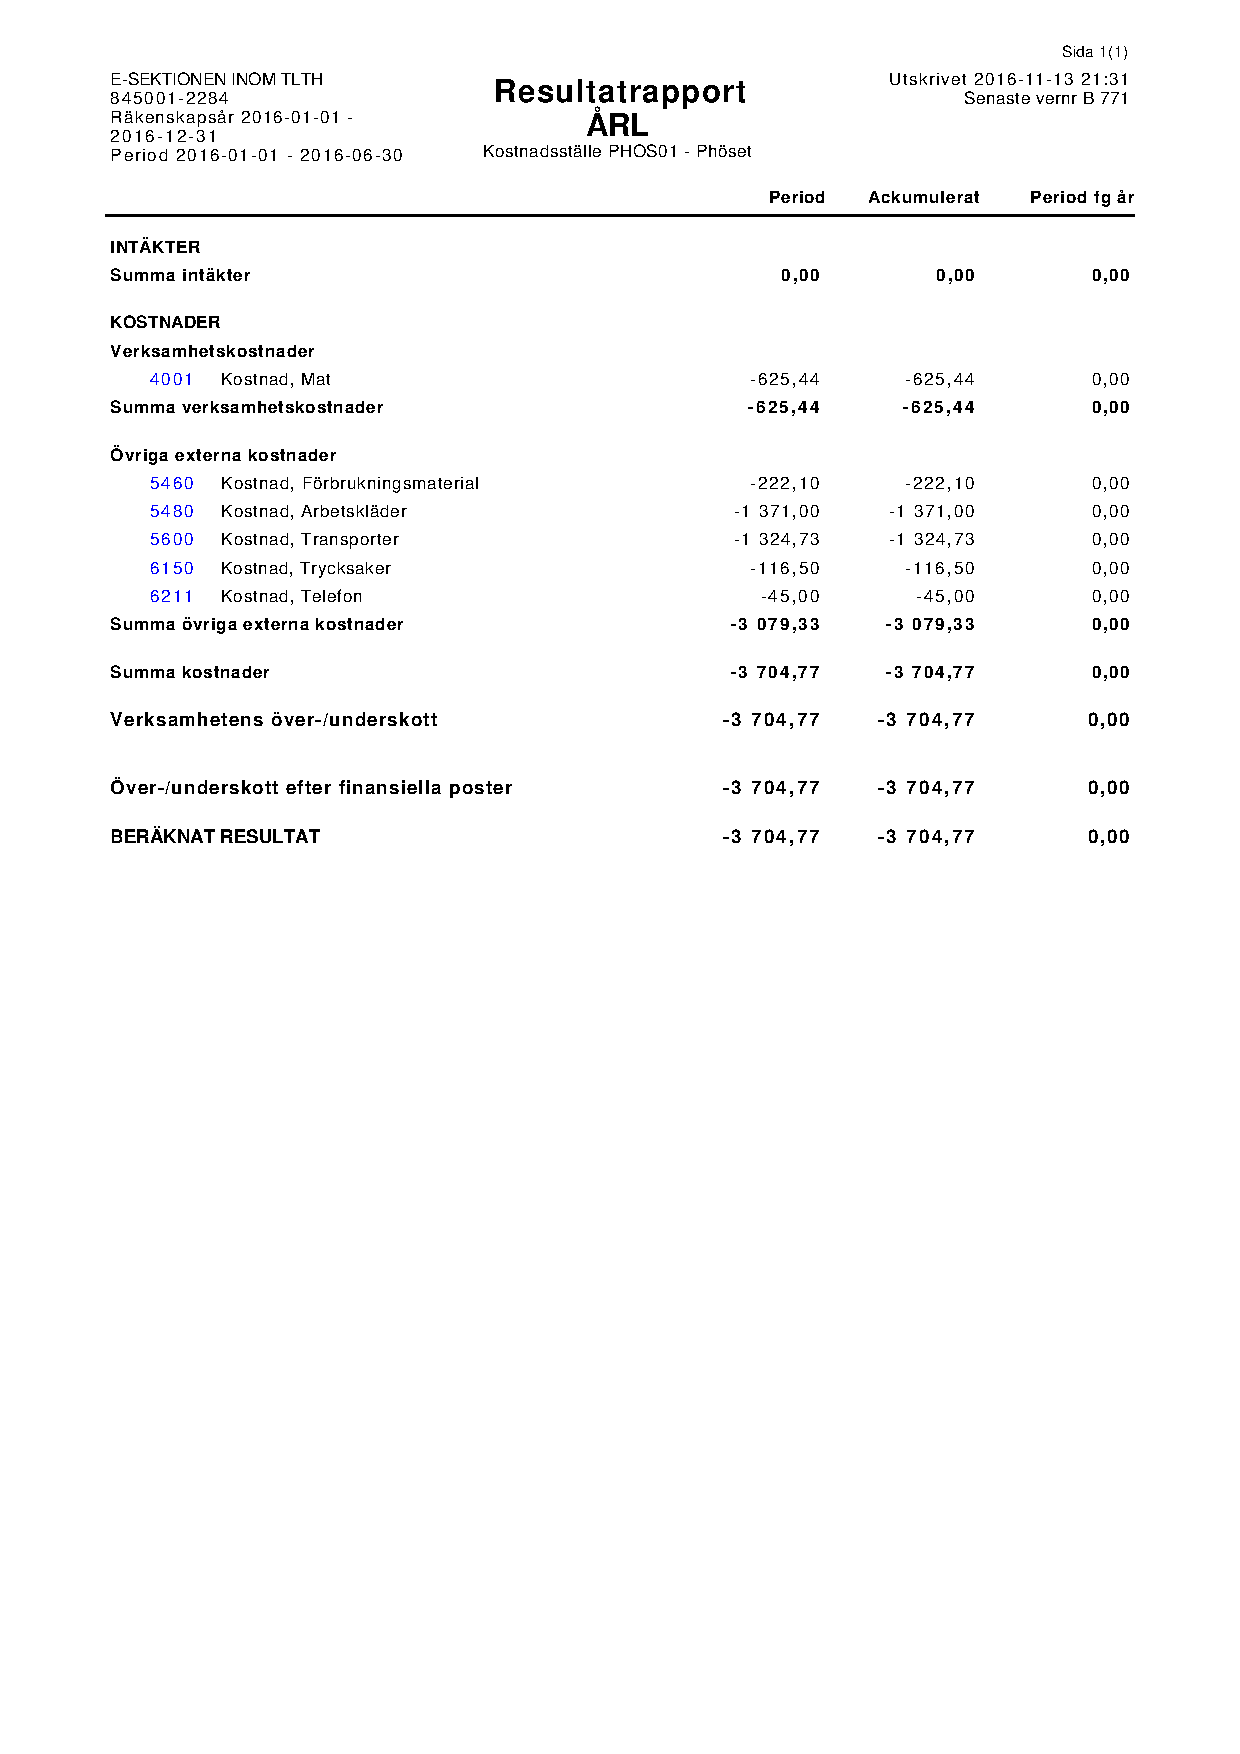
\includepdf[pages=-]{../_res/bokslut/phos01.pdf}
    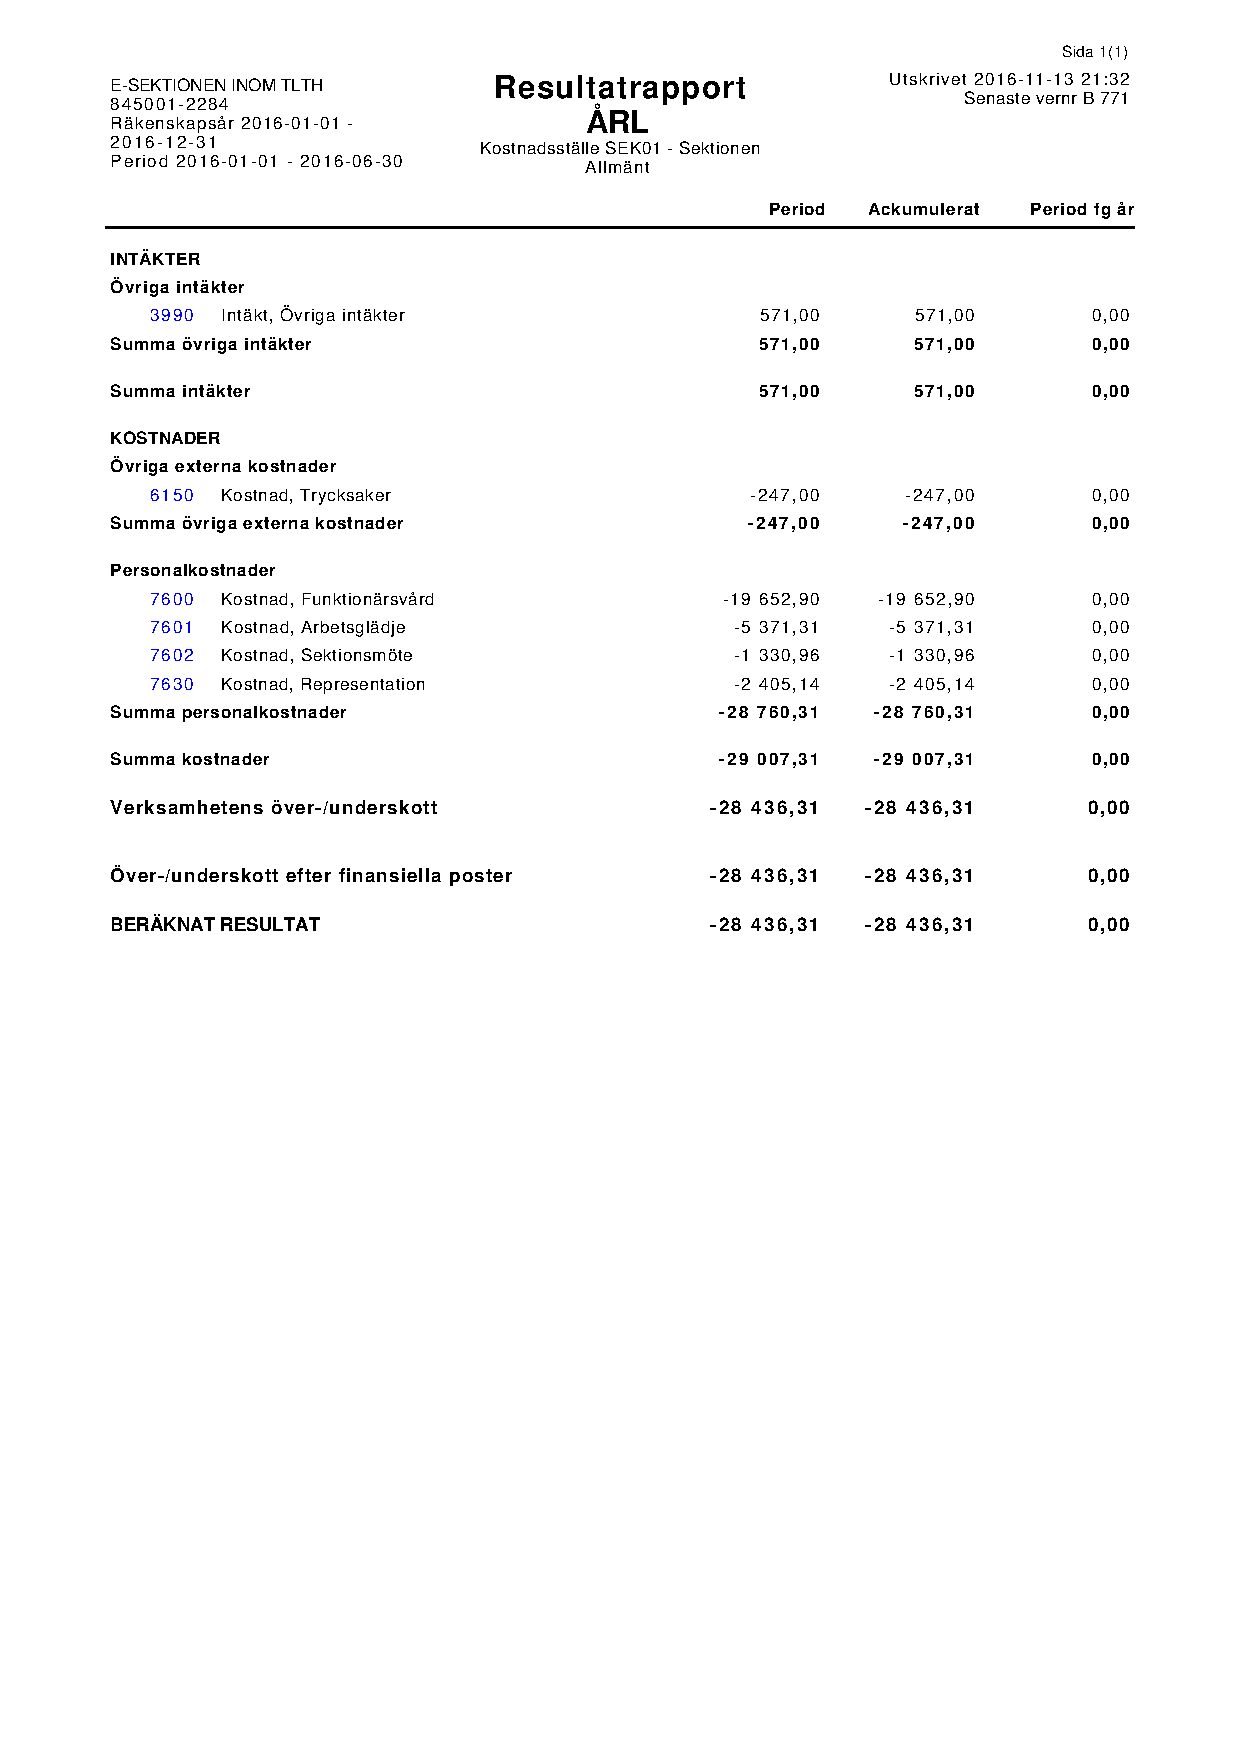
\includepdf[pages=-]{../_res/bokslut/sek01.pdf}
    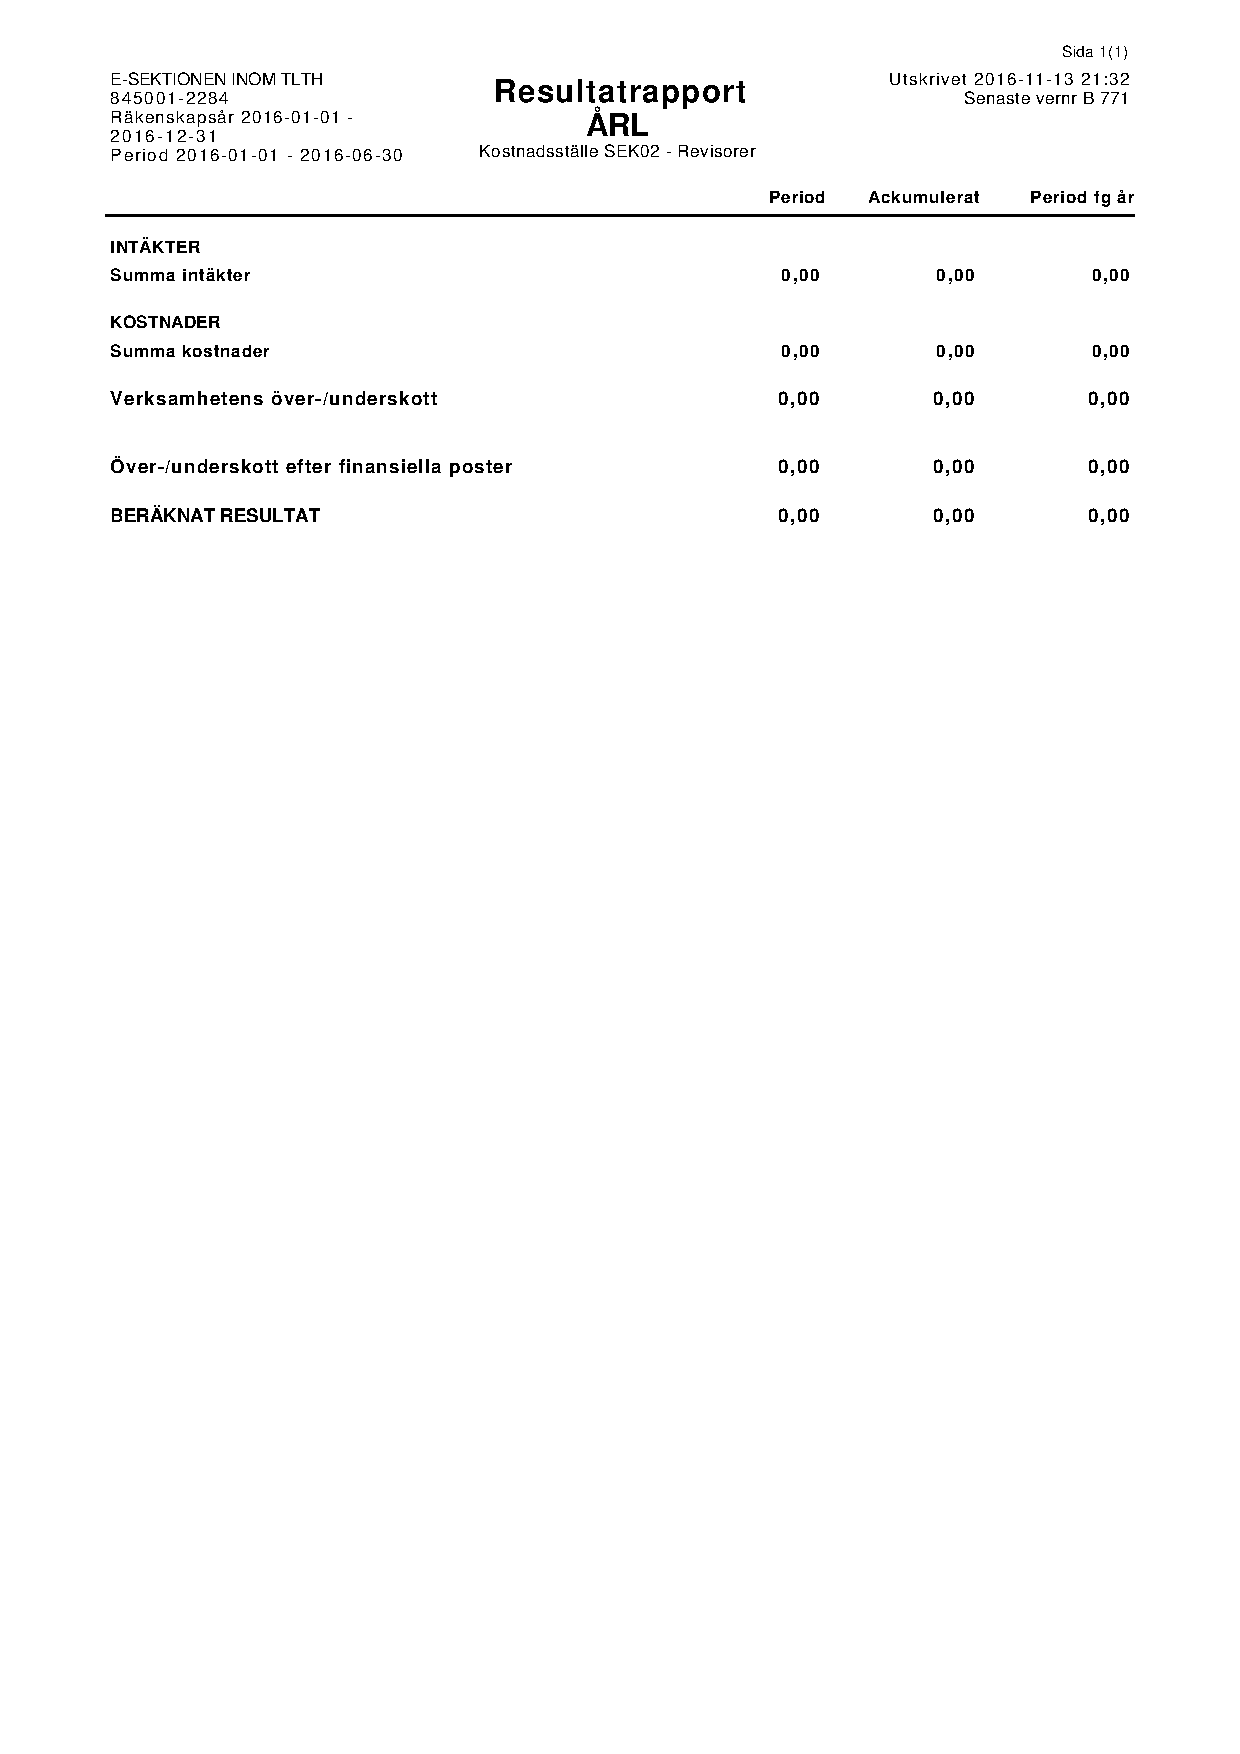
\includepdf[pages=-]{../_res/bokslut/sek02.pdf}
    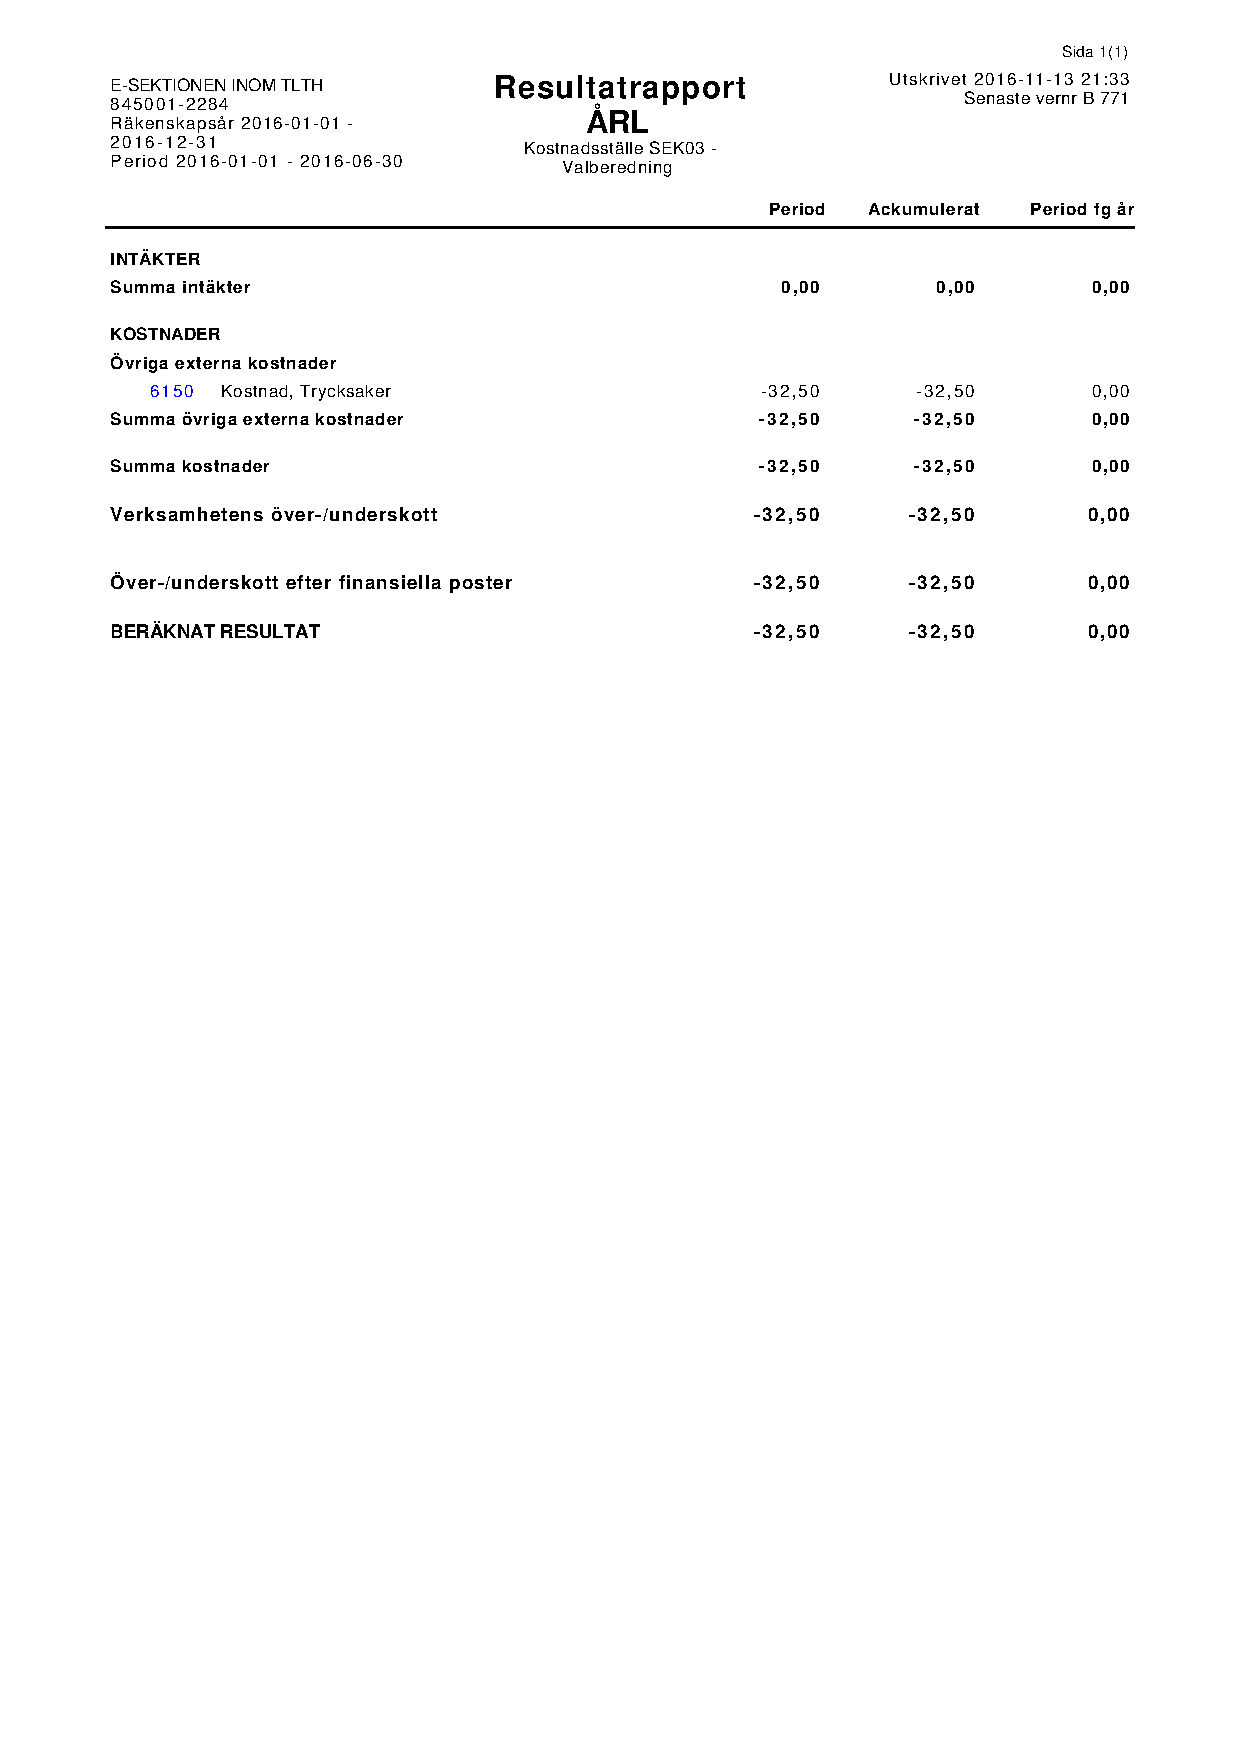
\includepdf[pages=-]{../_res/bokslut/sek04.pdf}
    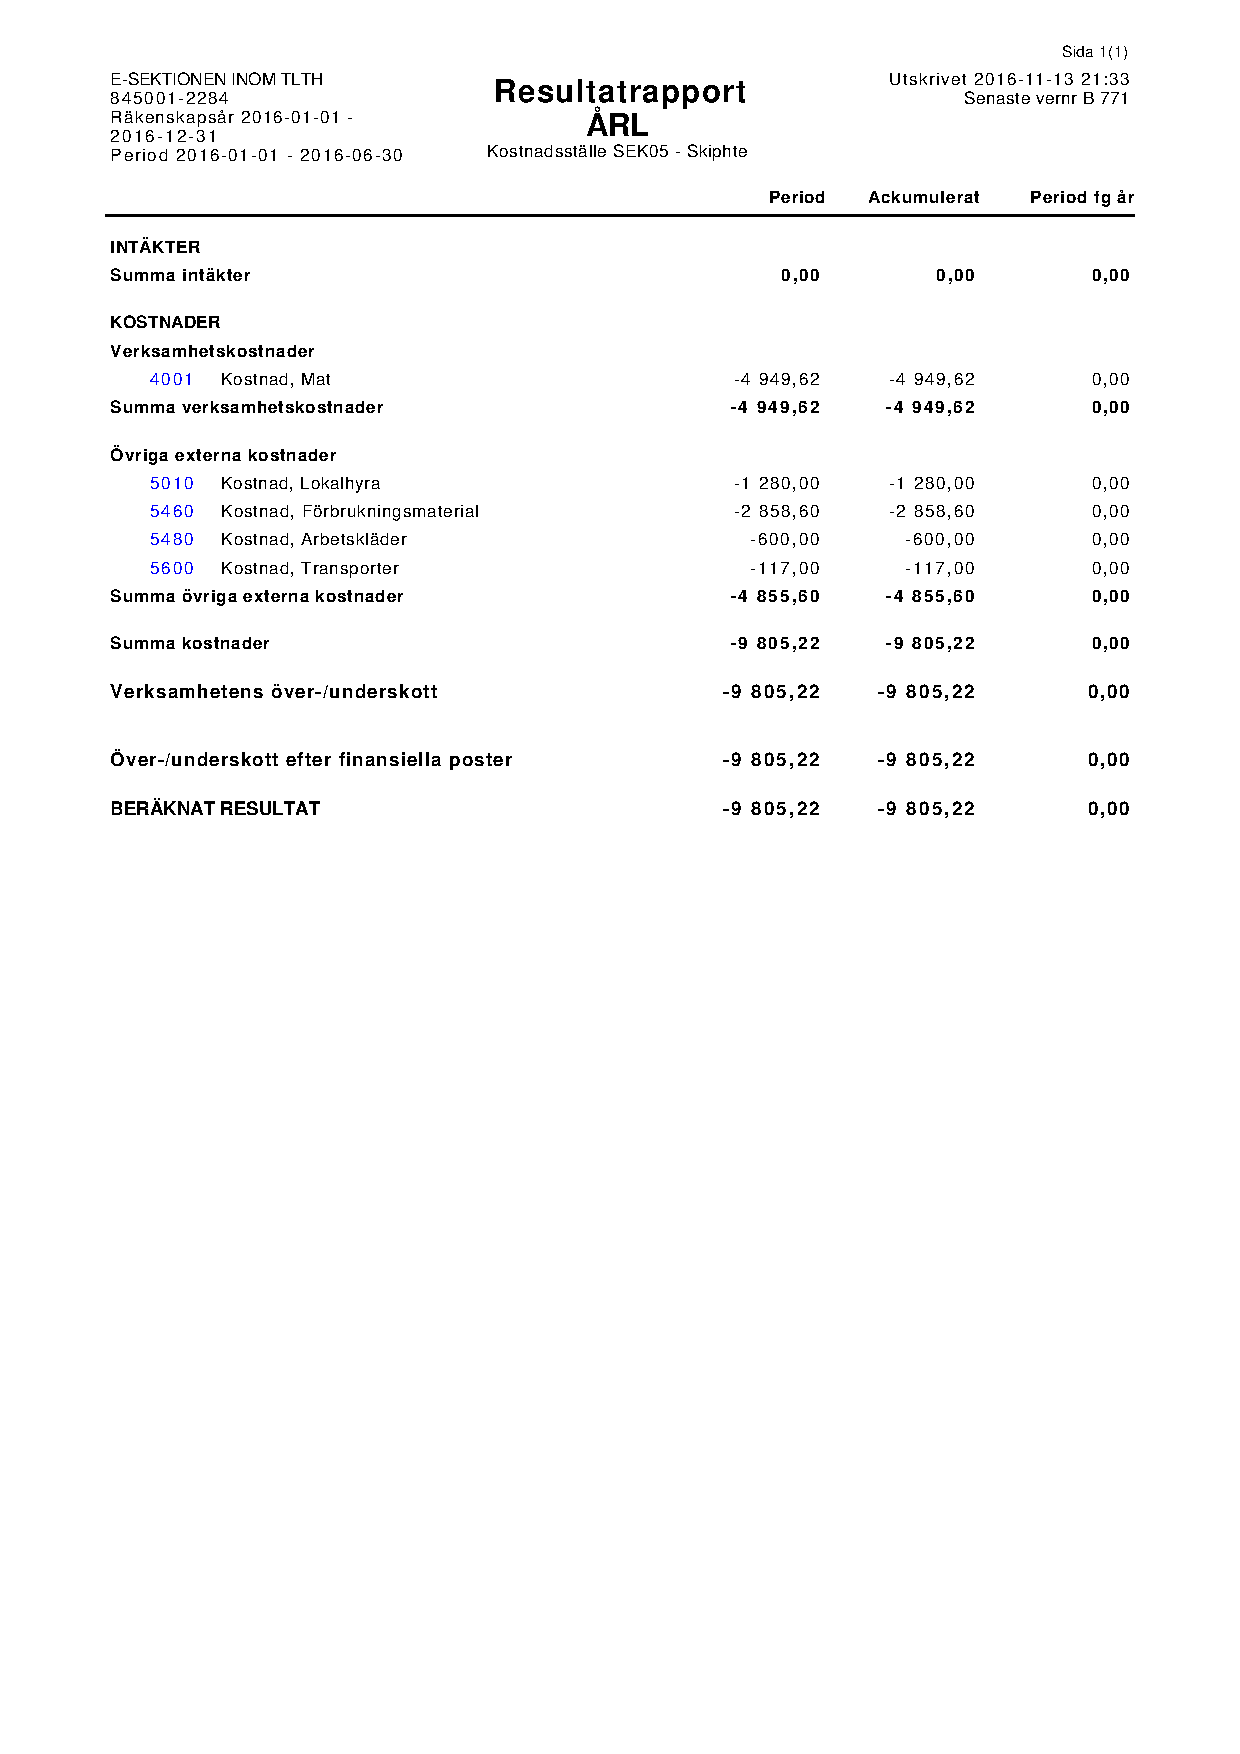
\includepdf[pages=-]{../_res/bokslut/sek05.pdf}
    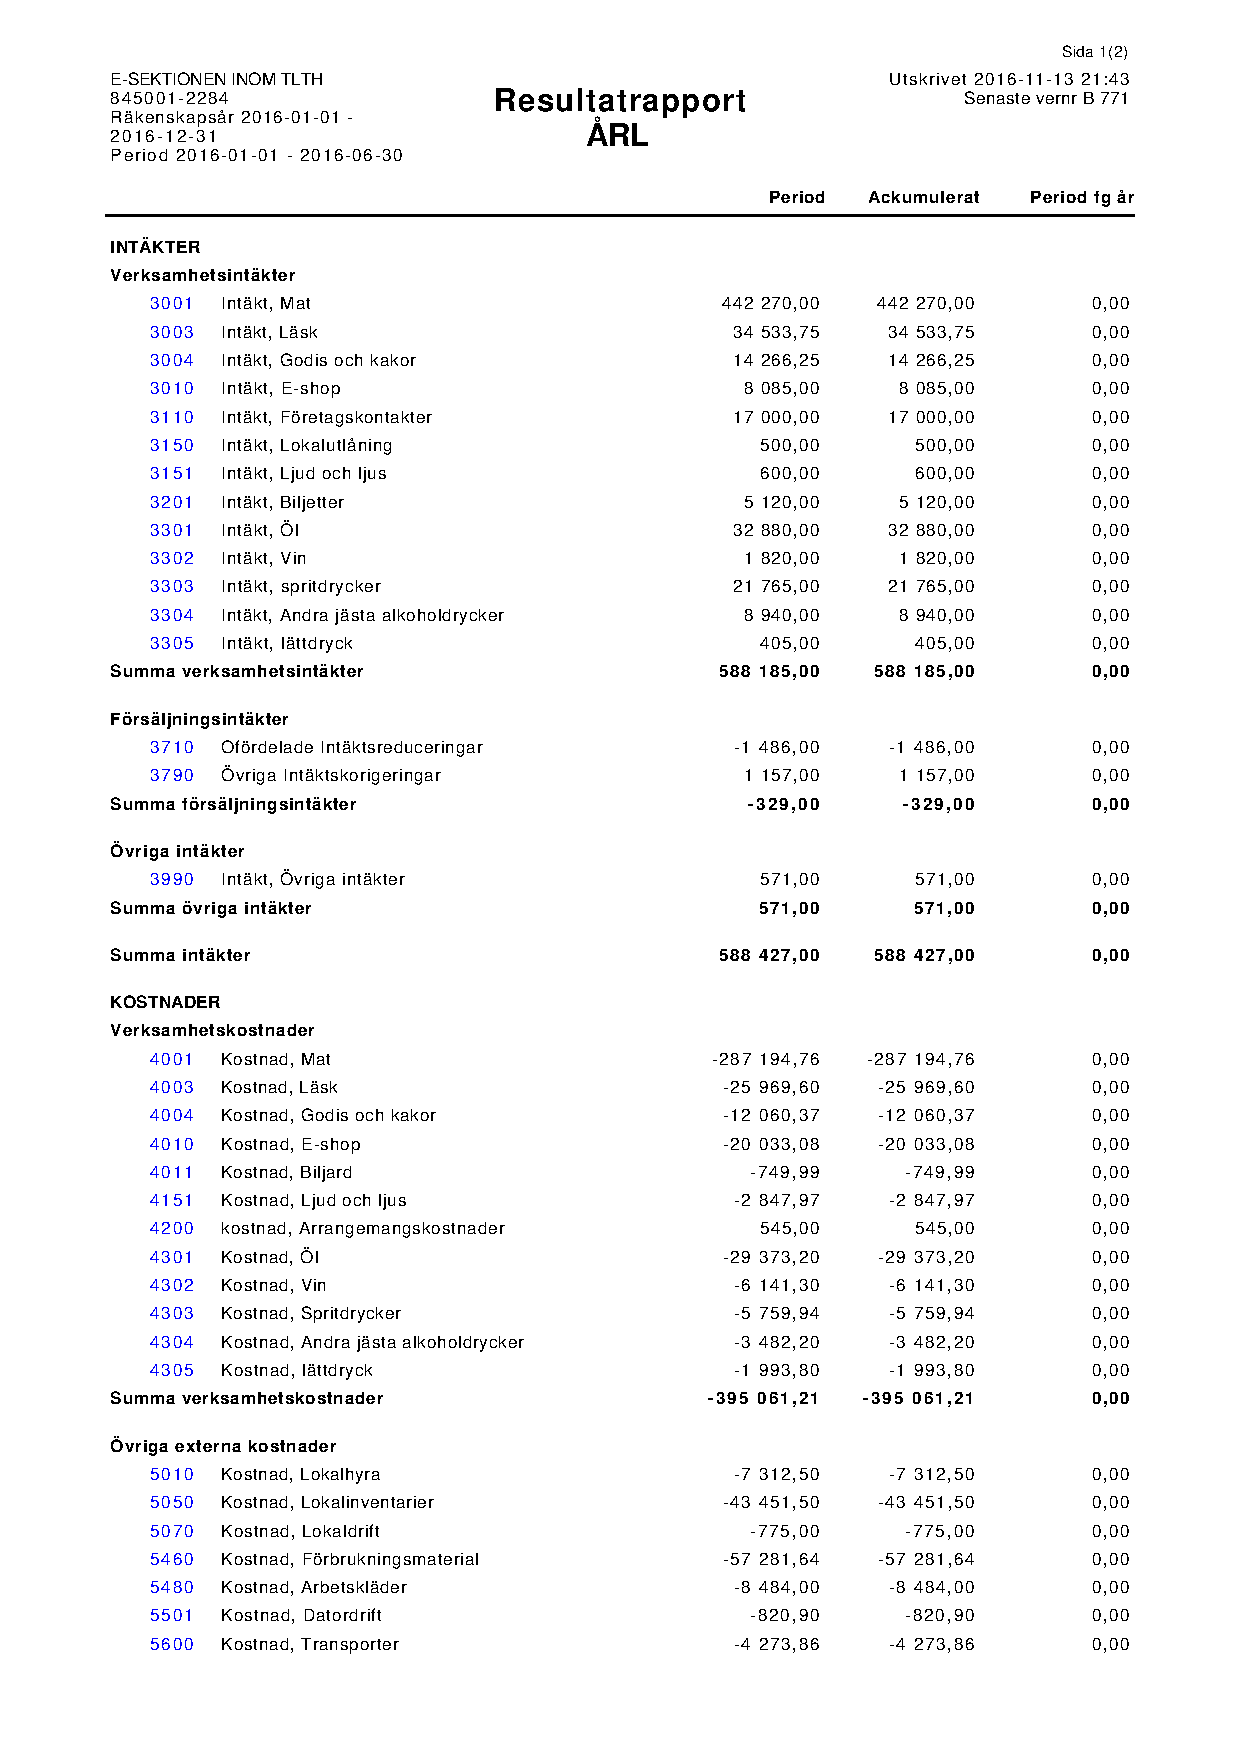
\includepdf[pages=-]{../_res/bokslut/sektionen.pdf}
    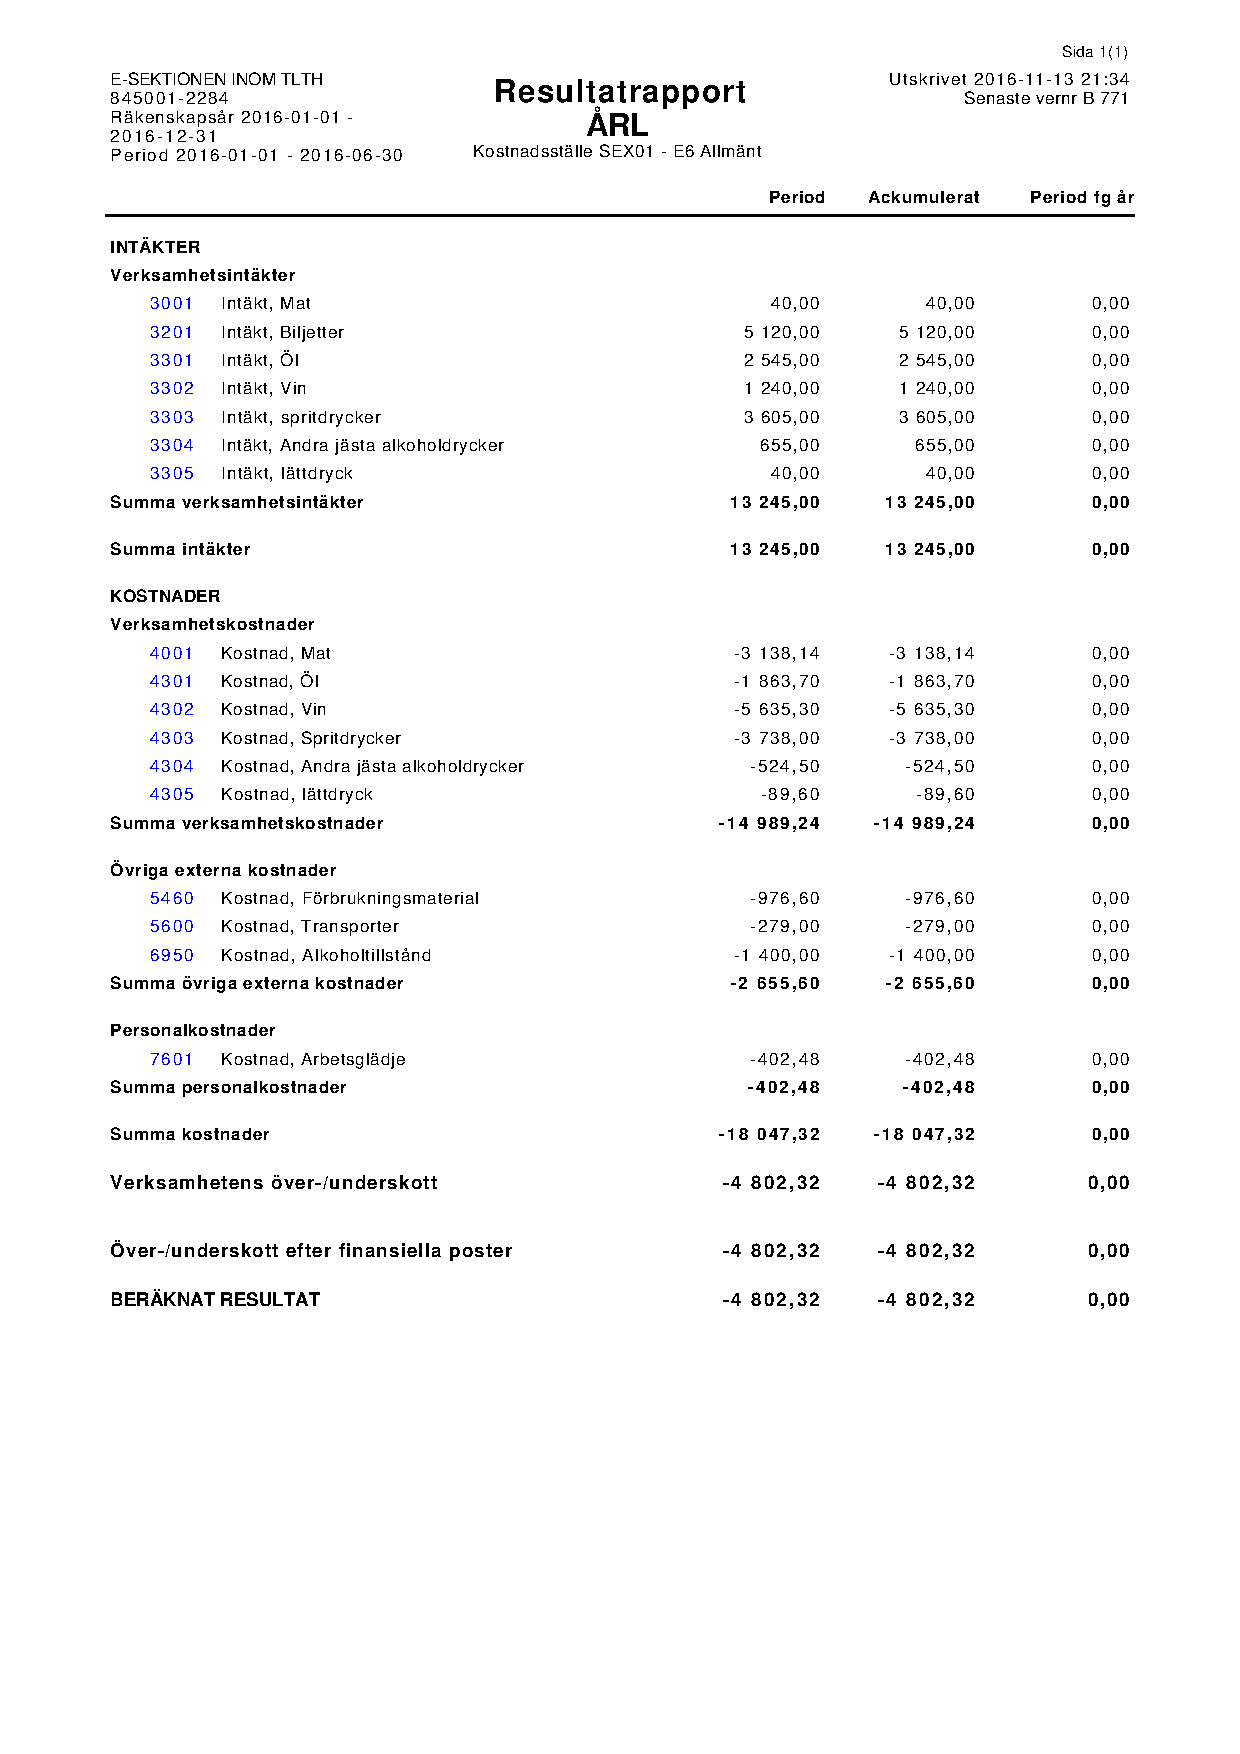
\includepdf[pages=-]{../_res/bokslut/sex01.pdf}
    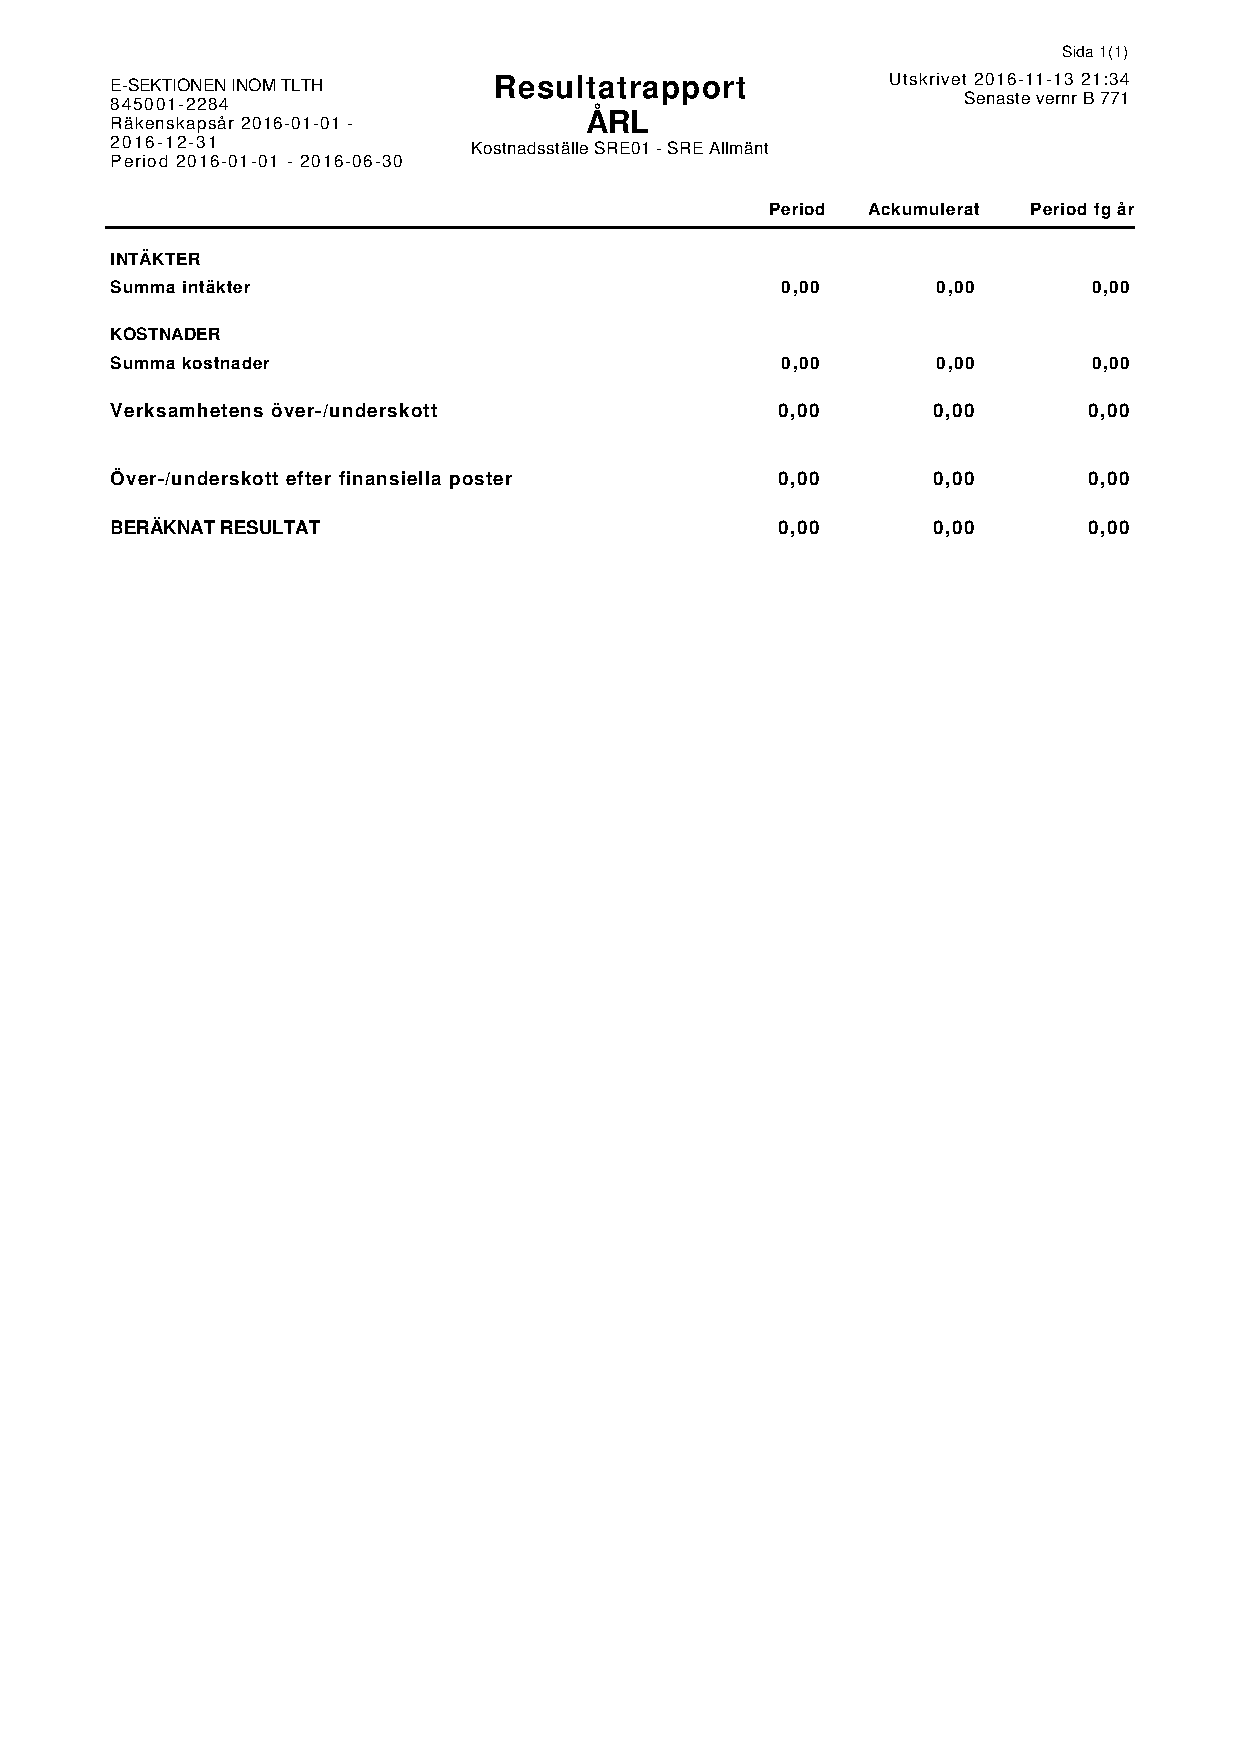
\includepdf[pages=-]{../_res/bokslut/sre01.pdf}
    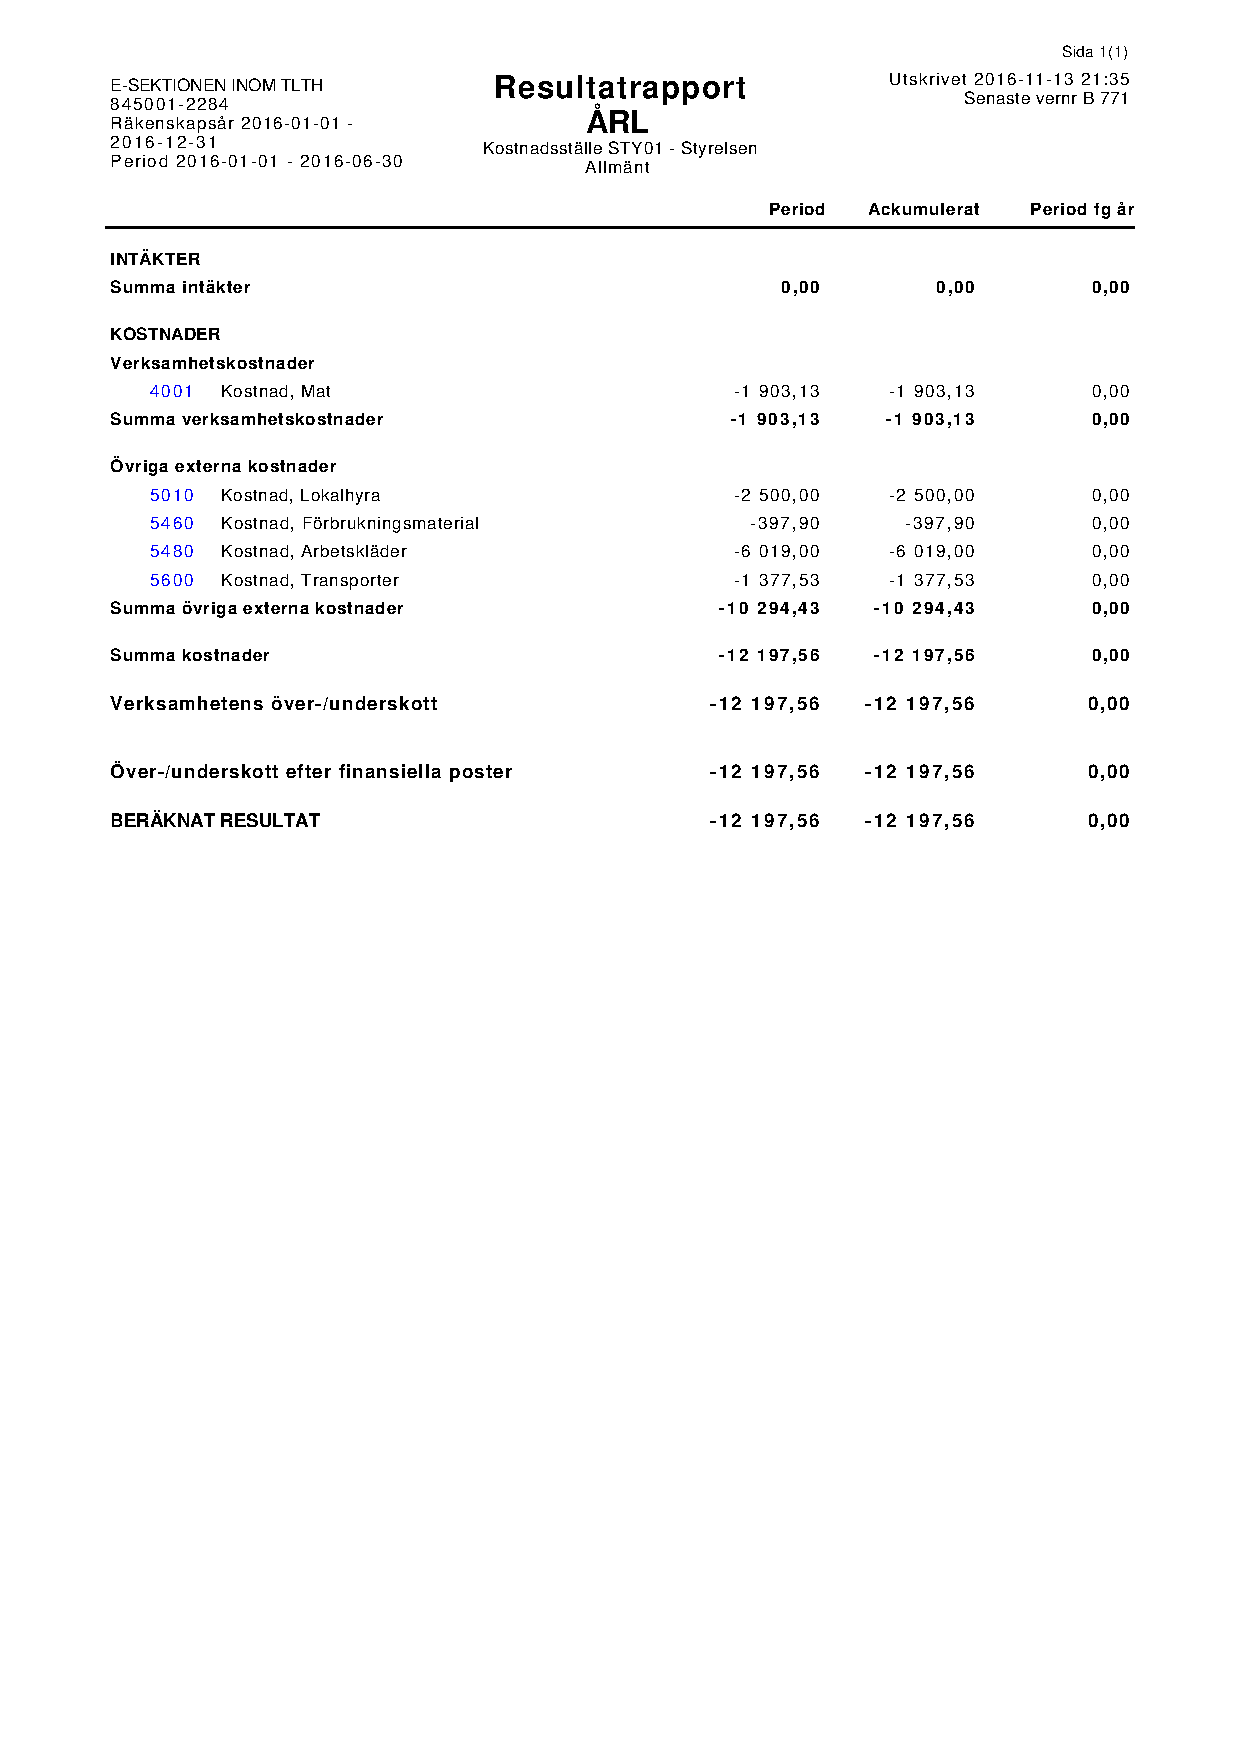
\includepdf[pages=-]{../_res/bokslut/sty01.pdf}
\end{supersection}
\end{comment}

\end{document}
